\documentclass[twoside]{book}

% Packages required by doxygen
\usepackage{calc}
\usepackage{doxygen}
\usepackage{graphicx}
\usepackage[utf8]{inputenc}
\usepackage{makeidx}
\usepackage{multicol}
\usepackage{multirow}
\usepackage{textcomp}
\usepackage[table]{xcolor}

% Font selection
\usepackage[T1]{fontenc}
\usepackage{mathptmx}
\usepackage[scaled=.90]{helvet}
\usepackage{courier}
\usepackage{amssymb}
\usepackage{sectsty}
\renewcommand{\familydefault}{\sfdefault}
\allsectionsfont{%
  \fontseries{bc}\selectfont%
  \color{darkgray}%
}
\renewcommand{\DoxyLabelFont}{%
  \fontseries{bc}\selectfont%
  \color{darkgray}%
}

% Page & text layout
\usepackage{geometry}
\geometry{%
  a4paper,%
  top=2.5cm,%
  bottom=2.5cm,%
  left=2.5cm,%
  right=2.5cm%
}
\tolerance=750
\hfuzz=15pt
\hbadness=750
\setlength{\emergencystretch}{15pt}
\setlength{\parindent}{0cm}
\setlength{\parskip}{0.2cm}
\makeatletter
\renewcommand{\paragraph}{%
  \@startsection{paragraph}{4}{0ex}{-1.0ex}{1.0ex}{%
    \normalfont\normalsize\bfseries\SS@parafont%
  }%
}
\renewcommand{\subparagraph}{%
  \@startsection{subparagraph}{5}{0ex}{-1.0ex}{1.0ex}{%
    \normalfont\normalsize\bfseries\SS@subparafont%
  }%
}
\makeatother

% Headers & footers
\usepackage{fancyhdr}
\pagestyle{fancyplain}
\fancyhead[LE]{\fancyplain{}{\bfseries\thepage}}
\fancyhead[CE]{\fancyplain{}{}}
\fancyhead[RE]{\fancyplain{}{\bfseries\leftmark}}
\fancyhead[LO]{\fancyplain{}{\bfseries\rightmark}}
\fancyhead[CO]{\fancyplain{}{}}
\fancyhead[RO]{\fancyplain{}{\bfseries\thepage}}
\fancyfoot[LE]{\fancyplain{}{}}
\fancyfoot[CE]{\fancyplain{}{}}
\fancyfoot[RE]{\fancyplain{}{\bfseries\scriptsize Generated on Mon Jun 20 2016 23\-:58\-:26 for tr\-I\-P\-S by Doxygen }}
\fancyfoot[LO]{\fancyplain{}{\bfseries\scriptsize Generated on Mon Jun 20 2016 23\-:58\-:26 for tr\-I\-P\-S by Doxygen }}
\fancyfoot[CO]{\fancyplain{}{}}
\fancyfoot[RO]{\fancyplain{}{}}
\renewcommand{\footrulewidth}{0.4pt}
\renewcommand{\chaptermark}[1]{%
  \markboth{#1}{}%
}
\renewcommand{\sectionmark}[1]{%
  \markright{\thesection\ #1}%
}

% Indices & bibliography
\usepackage{natbib}
\usepackage[titles]{tocloft}
\setcounter{tocdepth}{3}
\setcounter{secnumdepth}{5}
\makeindex

% Hyperlinks (required, but should be loaded last)
\usepackage{ifpdf}
\ifpdf
  \usepackage[pdftex,pagebackref=true]{hyperref}
\else
  \usepackage[ps2pdf,pagebackref=true]{hyperref}
\fi
\hypersetup{%
  colorlinks=true,%
  linkcolor=blue,%
  citecolor=blue,%
  unicode%
}

% Custom commands
\newcommand{\clearemptydoublepage}{%
  \newpage{\pagestyle{empty}\cleardoublepage}%
}


%===== C O N T E N T S =====

\begin{document}

% Titlepage & ToC
\hypersetup{pageanchor=false}
\pagenumbering{roman}
\begin{titlepage}
\vspace*{7cm}
\begin{center}%
{\Large tr\-I\-P\-S }\\
\vspace*{1cm}
{\large Generated by Doxygen 1.8.6}\\
\vspace*{0.5cm}
{\small Mon Jun 20 2016 23:58:26}\\
\end{center}
\end{titlepage}
\clearemptydoublepage
\tableofcontents
\clearemptydoublepage
\pagenumbering{arabic}
\hypersetup{pageanchor=true}

%--- Begin generated contents ---
\chapter{Namespace Index}
\section{Namespace List}
Here is a list of all documented namespaces with brief descriptions\-:\begin{DoxyCompactList}
\item\contentsline{section}{\hyperlink{namespacemodels}{models} \\*Contain all the model-\/class that will allow us an easy access from the rest of the code to the tables in our database }{\pageref{namespacemodels}}{}
\item\contentsline{section}{\hyperlink{namespaceurls}{urls} \\*This is the landing file of the A\-P\-I }{\pageref{namespaceurls}}{}
\item\contentsline{section}{\hyperlink{namespaceviews}{views} \\*Contain the M\-V\-C-\/view part.\-Each actions of the A\-P\-I land on a function stored in this file }{\pageref{namespaceviews}}{}
\end{DoxyCompactList}

\chapter{Hierarchical Index}
\section{Class Hierarchy}
This inheritance list is sorted roughly, but not completely, alphabetically\-:\begin{DoxyCompactList}
\item \contentsline{section}{com.\-example.\-fabien.\-lo53\-\_\-project.\-Example\-Unit\-Test}{\pageref{classcom_1_1example_1_1fabien_1_1lo53__project_1_1ExampleUnitTest}}{}
\item \contentsline{section}{ieee80211\-\_\-header}{\pageref{structieee80211__header}}{}
\item \contentsline{section}{ieee80211\-\_\-radiotap\-\_\-header}{\pageref{structieee80211__radiotap__header}}{}
\item Model\begin{DoxyCompactList}
\item \contentsline{section}{location.\-models.\-Calibration}{\pageref{classlocation_1_1models_1_1Calibration}}{}
\item \contentsline{section}{location.\-models.\-Device}{\pageref{classlocation_1_1models_1_1Device}}{}
\item \contentsline{section}{location.\-models.\-Location}{\pageref{classlocation_1_1models_1_1Location}}{}
\item \contentsline{section}{location.\-models.\-Measurement}{\pageref{classlocation_1_1models_1_1Measurement}}{}
\end{DoxyCompactList}
\item \contentsline{section}{com.\-example.\-fabien.\-lo53\-\_\-project.\-My\-Singleton}{\pageref{classcom_1_1example_1_1fabien_1_1lo53__project_1_1MySingleton}}{}
\item \contentsline{section}{radiotap\-\_\-align\-\_\-size}{\pageref{structradiotap__align__size}}{}
\item Runnable\begin{DoxyCompactList}
\item \contentsline{section}{com.\-example.\-fabien.\-lo53\-\_\-project.\-Display\-Toasts}{\pageref{classcom_1_1example_1_1fabien_1_1lo53__project_1_1DisplayToasts}}{}
\end{DoxyCompactList}
\item App\-Compat\-Activity\begin{DoxyCompactList}
\item \contentsline{section}{com.\-example.\-fabien.\-lo53\-\_\-project.\-Main\-Activity}{\pageref{classcom_1_1example_1_1fabien_1_1lo53__project_1_1MainActivity}}{}
\end{DoxyCompactList}
\item Application\-Test\-Case\begin{DoxyCompactList}
\item \contentsline{section}{com.\-example.\-fabien.\-lo53\-\_\-project.\-Application\-Test}{\pageref{classcom_1_1example_1_1fabien_1_1lo53__project_1_1ApplicationTest}}{}
\end{DoxyCompactList}
\end{DoxyCompactList}

\chapter{Class Index}
\section{Class List}
Here are the classes, structs, unions and interfaces with brief descriptions\-:\begin{DoxyCompactList}
\item\contentsline{section}{\hyperlink{classcom_1_1example_1_1fabien_1_1lo53__project_1_1ApplicationTest}{com.\-example.\-fabien.\-lo53\-\_\-project.\-Application\-Test} }{\pageref{classcom_1_1example_1_1fabien_1_1lo53__project_1_1ApplicationTest}}{}
\item\contentsline{section}{\hyperlink{classlocation_1_1models_1_1Calibration}{location.\-models.\-Calibration} \\*Class linked to the \hyperlink{classlocation_1_1models_1_1Calibration}{Calibration} table in the database }{\pageref{classlocation_1_1models_1_1Calibration}}{}
\item\contentsline{section}{\hyperlink{classlocation_1_1models_1_1Device}{location.\-models.\-Device} \\*Class linked to the \hyperlink{classlocation_1_1models_1_1Device}{Device} table in the database }{\pageref{classlocation_1_1models_1_1Device}}{}
\item\contentsline{section}{\hyperlink{classcom_1_1example_1_1fabien_1_1lo53__project_1_1DisplayToasts}{com.\-example.\-fabien.\-lo53\-\_\-project.\-Display\-Toasts} }{\pageref{classcom_1_1example_1_1fabien_1_1lo53__project_1_1DisplayToasts}}{}
\item\contentsline{section}{\hyperlink{classcom_1_1example_1_1fabien_1_1lo53__project_1_1ExampleUnitTest}{com.\-example.\-fabien.\-lo53\-\_\-project.\-Example\-Unit\-Test} }{\pageref{classcom_1_1example_1_1fabien_1_1lo53__project_1_1ExampleUnitTest}}{}
\item\contentsline{section}{\hyperlink{structieee80211__header}{ieee80211\-\_\-header} \\*I\-E\-E\-E 802.\-11 Header Header of protocol I\-E\-E\-E 802.\-11 }{\pageref{structieee80211__header}}{}
\item\contentsline{section}{\hyperlink{structieee80211__radiotap__header}{ieee80211\-\_\-radiotap\-\_\-header} \\*I\-E\-E\-E 802.\-11 Radiotap Header Header of radiotap protocol I\-E\-E\-E 802.\-11 }{\pageref{structieee80211__radiotap__header}}{}
\item\contentsline{section}{\hyperlink{classlocation_1_1models_1_1Location}{location.\-models.\-Location} \\*Class linked to the \hyperlink{classlocation_1_1models_1_1Location}{Location} table in the database }{\pageref{classlocation_1_1models_1_1Location}}{}
\item\contentsline{section}{\hyperlink{classcom_1_1example_1_1fabien_1_1lo53__project_1_1MainActivity}{com.\-example.\-fabien.\-lo53\-\_\-project.\-Main\-Activity} }{\pageref{classcom_1_1example_1_1fabien_1_1lo53__project_1_1MainActivity}}{}
\item\contentsline{section}{\hyperlink{classlocation_1_1models_1_1Measurement}{location.\-models.\-Measurement} \\*Class linked to the Measurment table in the database }{\pageref{classlocation_1_1models_1_1Measurement}}{}
\item\contentsline{section}{\hyperlink{classcom_1_1example_1_1fabien_1_1lo53__project_1_1MySingleton}{com.\-example.\-fabien.\-lo53\-\_\-project.\-My\-Singleton} }{\pageref{classcom_1_1example_1_1fabien_1_1lo53__project_1_1MySingleton}}{}
\item\contentsline{section}{\hyperlink{structradiotap__align__size}{radiotap\-\_\-align\-\_\-size} \\*Alignements and size of the radiotap header field From radiotap.\-c here \href{http://goo.gl/8pk0R9}{\tt http\-://goo.\-gl/8pk0\-R9} }{\pageref{structradiotap__align__size}}{}
\end{DoxyCompactList}

\chapter{File Index}
\section{File List}
Here is a list of all documented files with brief descriptions\-:\begin{DoxyCompactList}
\item\contentsline{section}{access-\/point/\hyperlink{app_8c}{app.\-c} \\*File that contains the main of the application }{\pageref{app_8c}}{}
\item\contentsline{section}{access-\/point/\hyperlink{http_8c}{http.\-c} \\*H\-T\-T\-P Functions }{\pageref{http_8c}}{}
\item\contentsline{section}{access-\/point/\hyperlink{http_8h}{http.\-h} \\*H\-T\-T\-P Functions }{\pageref{http_8h}}{}
\item\contentsline{section}{access-\/point/\hyperlink{mac_8c}{mac.\-c} \\*Usefull M\-A\-C Functions }{\pageref{mac_8c}}{}
\item\contentsline{section}{access-\/point/\hyperlink{mac_8h}{mac.\-h} \\*Usefull M\-A\-C Functions }{\pageref{mac_8h}}{}
\item\contentsline{section}{access-\/point/\hyperlink{pcap-thread_8c}{pcap-\/thread.\-c} \\*H\-T\-T\-P Stuff to deal with packets catched by libpcap }{\pageref{pcap-thread_8c}}{}
\item\contentsline{section}{access-\/point/\hyperlink{pcap-thread_8h}{pcap-\/thread.\-h} \\*H\-T\-T\-P Stuff to deal with packets catched by libpcap }{\pageref{pcap-thread_8h}}{}
\end{DoxyCompactList}

\chapter{Namespace Documentation}
\hypertarget{namespacemodels}{\section{models Namespace Reference}
\label{namespacemodels}\index{models@{models}}
}


Contain all the model-\/class that will allow us an easy access from the rest of the code to the tables in our database.  




\subsection{Detailed Description}
Contain all the model-\/class that will allow us an easy access from the rest of the code to the tables in our database. 
\hypertarget{namespaceurls}{\section{urls Namespace Reference}
\label{namespaceurls}\index{urls@{urls}}
}


This is the landing file of the A\-P\-I.  




\subsection{Detailed Description}
This is the landing file of the A\-P\-I. Every U\-R\-Ls are defines here and will redirect to a specific view. 
\hypertarget{namespaceviews}{\section{views Namespace Reference}
\label{namespaceviews}\index{views@{views}}
}


Contain the M\-V\-C-\/view part.\-Each actions of the A\-P\-I land on a function stored in this file.  




\subsection{Detailed Description}
Contain the M\-V\-C-\/view part.\-Each actions of the A\-P\-I land on a function stored in this file. 
\chapter{Class Documentation}
\hypertarget{classcom_1_1example_1_1fabien_1_1lo53__project_1_1ApplicationTest}{\section{com.\-example.\-fabien.\-lo53\-\_\-project.\-Application\-Test Class Reference}
\label{classcom_1_1example_1_1fabien_1_1lo53__project_1_1ApplicationTest}\index{com.\-example.\-fabien.\-lo53\-\_\-project.\-Application\-Test@{com.\-example.\-fabien.\-lo53\-\_\-project.\-Application\-Test}}
}
Inheritance diagram for com.\-example.\-fabien.\-lo53\-\_\-project.\-Application\-Test\-:\begin{figure}[H]
\begin{center}
\leavevmode
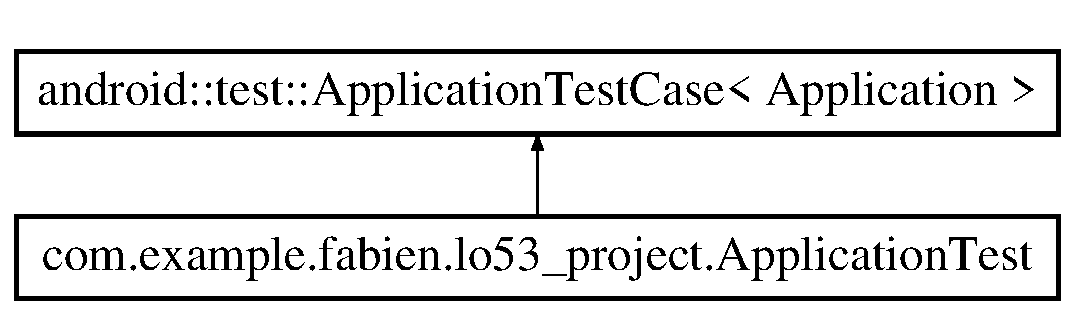
\includegraphics[height=2.000000cm]{classcom_1_1example_1_1fabien_1_1lo53__project_1_1ApplicationTest}
\end{center}
\end{figure}


\subsection{Detailed Description}
\href{http://d.android.com/tools/testing/testing_android.html}{\tt Testing Fundamentals} 

The documentation for this class was generated from the following file\-:\begin{DoxyCompactItemize}
\item 
appli/app/src/android\-Test/java/com/example/fabien/lo53\-\_\-project/Application\-Test.\-java\end{DoxyCompactItemize}

\hypertarget{classlocation_1_1models_1_1Calibration}{\section{location.\-models.\-Calibration Class Reference}
\label{classlocation_1_1models_1_1Calibration}\index{location.\-models.\-Calibration@{location.\-models.\-Calibration}}
}


Class linked to the \hyperlink{classlocation_1_1models_1_1Calibration}{Calibration} table in the database.  


Inheritance diagram for location.\-models.\-Calibration\-:\begin{figure}[H]
\begin{center}
\leavevmode
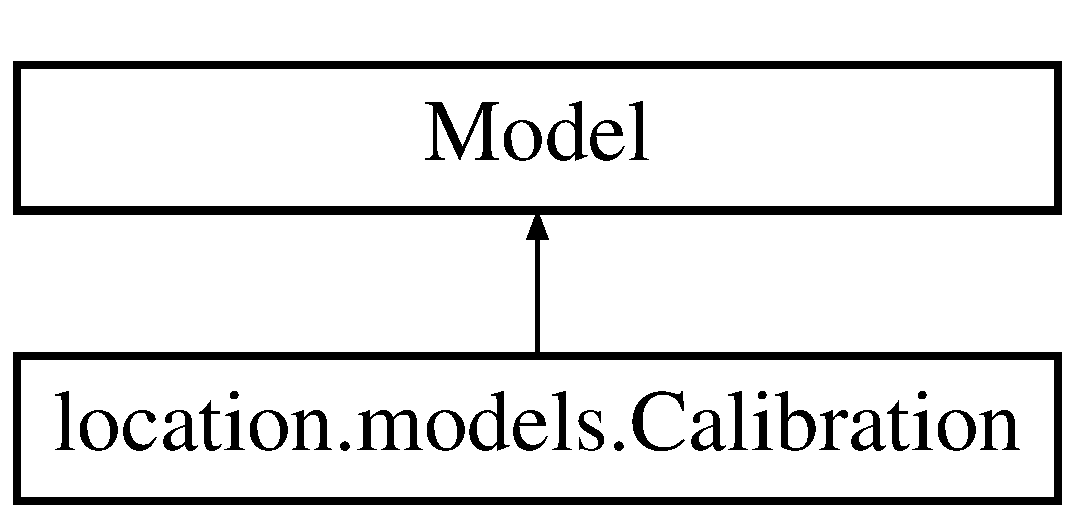
\includegraphics[height=2.000000cm]{classlocation_1_1models_1_1Calibration}
\end{center}
\end{figure}
\subsection*{Static Public Attributes}
\begin{DoxyCompactItemize}
\item 
\hypertarget{classlocation_1_1models_1_1Calibration_a60d6df8ce1d7517f7f30b068db0ae321}{tuple {\bfseries loc\-\_\-id} = models.\-Foreign\-Key(\hyperlink{classlocation_1_1models_1_1Location}{Location}, on\-\_\-delete=models.\-C\-A\-S\-C\-A\-D\-E)}\label{classlocation_1_1models_1_1Calibration_a60d6df8ce1d7517f7f30b068db0ae321}

\item 
\hypertarget{classlocation_1_1models_1_1Calibration_ab8dd1e6169ab87e10ba1063f5e308d6d}{tuple {\bfseries ss\-\_\-value} = models.\-Float\-Field(default=0)}\label{classlocation_1_1models_1_1Calibration_ab8dd1e6169ab87e10ba1063f5e308d6d}

\item 
\hypertarget{classlocation_1_1models_1_1Calibration_a30217d1b23c0d4b8def552ddd1d2eb6c}{tuple {\bfseries ap\-\_\-id} = models.\-Integer\-Field(default=0)}\label{classlocation_1_1models_1_1Calibration_a30217d1b23c0d4b8def552ddd1d2eb6c}

\end{DoxyCompactItemize}


\subsection{Detailed Description}
Class linked to the \hyperlink{classlocation_1_1models_1_1Calibration}{Calibration} table in the database. 

The documentation for this class was generated from the following file\-:\begin{DoxyCompactItemize}
\item 
server/location/models.\-py\end{DoxyCompactItemize}

\hypertarget{classlocation_1_1models_1_1Device}{\section{location.\-models.\-Device Class Reference}
\label{classlocation_1_1models_1_1Device}\index{location.\-models.\-Device@{location.\-models.\-Device}}
}


Class linked to the \hyperlink{classlocation_1_1models_1_1Device}{Device} table in the database.  


Inheritance diagram for location.\-models.\-Device\-:\begin{figure}[H]
\begin{center}
\leavevmode
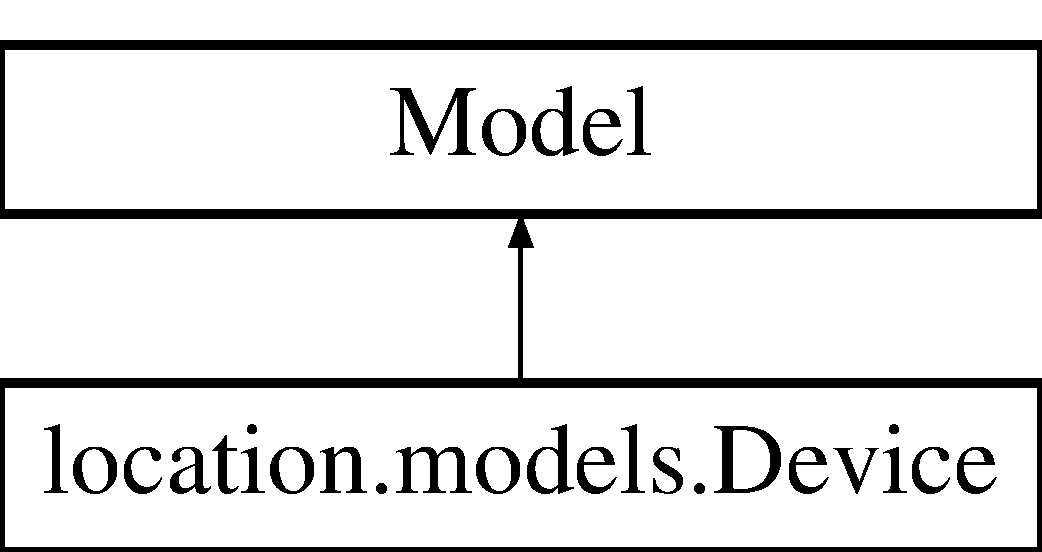
\includegraphics[height=2.000000cm]{classlocation_1_1models_1_1Device}
\end{center}
\end{figure}
\subsection*{Static Public Member Functions}
\begin{DoxyCompactItemize}
\item 
\hypertarget{classlocation_1_1models_1_1Device_a45fa946e37903d6515ec4b2237e7e429}{def {\bfseries get\-\_\-macs}}\label{classlocation_1_1models_1_1Device_a45fa946e37903d6515ec4b2237e7e429}

\end{DoxyCompactItemize}
\subsection*{Static Public Attributes}
\begin{DoxyCompactItemize}
\item 
\hypertarget{classlocation_1_1models_1_1Device_af0b3482b70bc9eefc334a1a211dddb02}{tuple {\bfseries mac} = models.\-Char\-Field(max\-\_\-length=255)}\label{classlocation_1_1models_1_1Device_af0b3482b70bc9eefc334a1a211dddb02}

\item 
\hypertarget{classlocation_1_1models_1_1Device_a89ef52d772d03025f287453bb8e39e43}{tuple {\bfseries calibration} = models.\-Boolean\-Field(default=0)}\label{classlocation_1_1models_1_1Device_a89ef52d772d03025f287453bb8e39e43}

\end{DoxyCompactItemize}


\subsection{Detailed Description}
Class linked to the \hyperlink{classlocation_1_1models_1_1Device}{Device} table in the database. 

The documentation for this class was generated from the following file\-:\begin{DoxyCompactItemize}
\item 
server/location/models.\-py\end{DoxyCompactItemize}

\hypertarget{classcom_1_1example_1_1fabien_1_1lo53__project_1_1DisplayToasts}{\section{com.\-example.\-fabien.\-lo53\-\_\-project.\-Display\-Toasts Class Reference}
\label{classcom_1_1example_1_1fabien_1_1lo53__project_1_1DisplayToasts}\index{com.\-example.\-fabien.\-lo53\-\_\-project.\-Display\-Toasts@{com.\-example.\-fabien.\-lo53\-\_\-project.\-Display\-Toasts}}
}
Inheritance diagram for com.\-example.\-fabien.\-lo53\-\_\-project.\-Display\-Toasts\-:\begin{figure}[H]
\begin{center}
\leavevmode
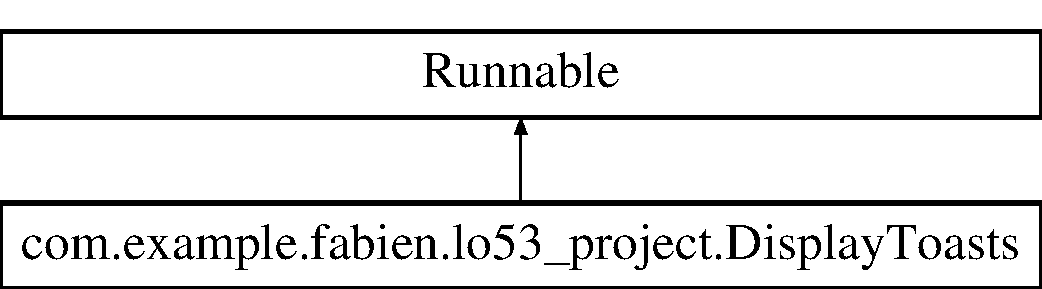
\includegraphics[height=2.000000cm]{classcom_1_1example_1_1fabien_1_1lo53__project_1_1DisplayToasts}
\end{center}
\end{figure}
\subsection*{Public Member Functions}
\begin{DoxyCompactItemize}
\item 
\hypertarget{classcom_1_1example_1_1fabien_1_1lo53__project_1_1DisplayToasts_a8161863a82db4f434348d4a977b3099e}{{\bfseries Display\-Toasts} (Context m\-Context, String text)}\label{classcom_1_1example_1_1fabien_1_1lo53__project_1_1DisplayToasts_a8161863a82db4f434348d4a977b3099e}

\item 
\hypertarget{classcom_1_1example_1_1fabien_1_1lo53__project_1_1DisplayToasts_a84a5d7dc4f9da4c7cf28e15c3f43b805}{void {\bfseries run} ()}\label{classcom_1_1example_1_1fabien_1_1lo53__project_1_1DisplayToasts_a84a5d7dc4f9da4c7cf28e15c3f43b805}

\end{DoxyCompactItemize}


\subsection{Detailed Description}
Created by Fabien on 27/05/2016. 

The documentation for this class was generated from the following file\-:\begin{DoxyCompactItemize}
\item 
appli/app/src/main/java/com/example/fabien/lo53\-\_\-project/Display\-Toasts.\-java\end{DoxyCompactItemize}

\hypertarget{classcom_1_1example_1_1fabien_1_1lo53__project_1_1ExampleUnitTest}{\section{com.\-example.\-fabien.\-lo53\-\_\-project.\-Example\-Unit\-Test Class Reference}
\label{classcom_1_1example_1_1fabien_1_1lo53__project_1_1ExampleUnitTest}\index{com.\-example.\-fabien.\-lo53\-\_\-project.\-Example\-Unit\-Test@{com.\-example.\-fabien.\-lo53\-\_\-project.\-Example\-Unit\-Test}}
}
\subsection*{Public Member Functions}
\begin{DoxyCompactItemize}
\item 
\hypertarget{classcom_1_1example_1_1fabien_1_1lo53__project_1_1ExampleUnitTest_aa992fe18142b77ce997ac20ecbc0d2ed}{void {\bfseries addition\-\_\-is\-Correct} ()  throws Exception }\label{classcom_1_1example_1_1fabien_1_1lo53__project_1_1ExampleUnitTest_aa992fe18142b77ce997ac20ecbc0d2ed}

\end{DoxyCompactItemize}


\subsection{Detailed Description}
To work on unit tests, switch the Test Artifact in the Build Variants view. 

The documentation for this class was generated from the following file\-:\begin{DoxyCompactItemize}
\item 
appli/app/src/test/java/com/example/fabien/lo53\-\_\-project/Example\-Unit\-Test.\-java\end{DoxyCompactItemize}

\hypertarget{structieee80211__header}{\section{ieee80211\-\_\-header Struct Reference}
\label{structieee80211__header}\index{ieee80211\-\_\-header@{ieee80211\-\_\-header}}
}


I\-E\-E\-E 802.\-11 Header Header of protocol I\-E\-E\-E 802.\-11.  




{\ttfamily \#include $<$pcap-\/thread.\-h$>$}

\subsection*{Public Attributes}
\begin{DoxyCompactItemize}
\item 
\hypertarget{structieee80211__header_aaa9c4e9502842e191a237ee80f89c292}{u\-\_\-short {\bfseries frame\-\_\-control}}\label{structieee80211__header_aaa9c4e9502842e191a237ee80f89c292}

\item 
\hypertarget{structieee80211__header_aff9ef1a16cd65df85e6abd03835cc2df}{u\-\_\-short {\bfseries frame\-\_\-duration}}\label{structieee80211__header_aff9ef1a16cd65df85e6abd03835cc2df}

\item 
\hypertarget{structieee80211__header_ad269c3c4354cbde2864c44fc9584d929}{u\-\_\-char {\bfseries recipient} \mbox{[}6\mbox{]}}\label{structieee80211__header_ad269c3c4354cbde2864c44fc9584d929}

\item 
\hypertarget{structieee80211__header_afbd721b7ef6d4202ebc83f0e6a68742e}{u\-\_\-char {\bfseries source\-\_\-addr} \mbox{[}6\mbox{]}}\label{structieee80211__header_afbd721b7ef6d4202ebc83f0e6a68742e}

\item 
\hypertarget{structieee80211__header_a0f804665fc1f60a1cdc868804dd54e94}{u\-\_\-char {\bfseries address3} \mbox{[}6\mbox{]}}\label{structieee80211__header_a0f804665fc1f60a1cdc868804dd54e94}

\item 
\hypertarget{structieee80211__header_a43c2294d4f1591916910da93f8813ec6}{u\-\_\-short {\bfseries sequence\-\_\-control}}\label{structieee80211__header_a43c2294d4f1591916910da93f8813ec6}

\item 
\hypertarget{structieee80211__header_a54150ad91cd2d9f21e3a8719fffdbc56}{u\-\_\-char {\bfseries address4} \mbox{[}6\mbox{]}}\label{structieee80211__header_a54150ad91cd2d9f21e3a8719fffdbc56}

\end{DoxyCompactItemize}


\subsection{Detailed Description}
I\-E\-E\-E 802.\-11 Header Header of protocol I\-E\-E\-E 802.\-11. 

The documentation for this struct was generated from the following file\-:\begin{DoxyCompactItemize}
\item 
access-\/point/\hyperlink{pcap-thread_8h}{pcap-\/thread.\-h}\end{DoxyCompactItemize}

\hypertarget{structieee80211__radiotap__header}{\section{ieee80211\-\_\-radiotap\-\_\-header Struct Reference}
\label{structieee80211__radiotap__header}\index{ieee80211\-\_\-radiotap\-\_\-header@{ieee80211\-\_\-radiotap\-\_\-header}}
}


I\-E\-E\-E 802.\-11 Radiotap Header Header of radiotap protocol I\-E\-E\-E 802.\-11.  




{\ttfamily \#include $<$pcap-\/thread.\-h$>$}

\subsection*{Public Attributes}
\begin{DoxyCompactItemize}
\item 
\hypertarget{structieee80211__radiotap__header_a0c2d940a5b3d413e6beaa30cbe192943}{u\-\_\-char {\bfseries it\-\_\-version}}\label{structieee80211__radiotap__header_a0c2d940a5b3d413e6beaa30cbe192943}

\item 
\hypertarget{structieee80211__radiotap__header_a197bc8ad9b9ff289c17b97e2f4738f1f}{u\-\_\-char {\bfseries it\-\_\-pad}}\label{structieee80211__radiotap__header_a197bc8ad9b9ff289c17b97e2f4738f1f}

\item 
\hypertarget{structieee80211__radiotap__header_a947c98f2b58051ca730dea2ede65d091}{u\-\_\-char {\bfseries it\-\_\-len} \mbox{[}2\mbox{]}}\label{structieee80211__radiotap__header_a947c98f2b58051ca730dea2ede65d091}

\item 
\hypertarget{structieee80211__radiotap__header_a4a46520e815e3d2b7892ecfce6412693}{u\-\_\-char {\bfseries it\-\_\-present} \mbox{[}4\mbox{]}}\label{structieee80211__radiotap__header_a4a46520e815e3d2b7892ecfce6412693}

\end{DoxyCompactItemize}


\subsection{Detailed Description}
I\-E\-E\-E 802.\-11 Radiotap Header Header of radiotap protocol I\-E\-E\-E 802.\-11. 

The documentation for this struct was generated from the following file\-:\begin{DoxyCompactItemize}
\item 
access-\/point/\hyperlink{pcap-thread_8h}{pcap-\/thread.\-h}\end{DoxyCompactItemize}

\hypertarget{classlocation_1_1models_1_1Location}{\section{location.\-models.\-Location Class Reference}
\label{classlocation_1_1models_1_1Location}\index{location.\-models.\-Location@{location.\-models.\-Location}}
}


Class linked to the \hyperlink{classlocation_1_1models_1_1Location}{Location} table in the database.  


Inheritance diagram for location.\-models.\-Location\-:\begin{figure}[H]
\begin{center}
\leavevmode
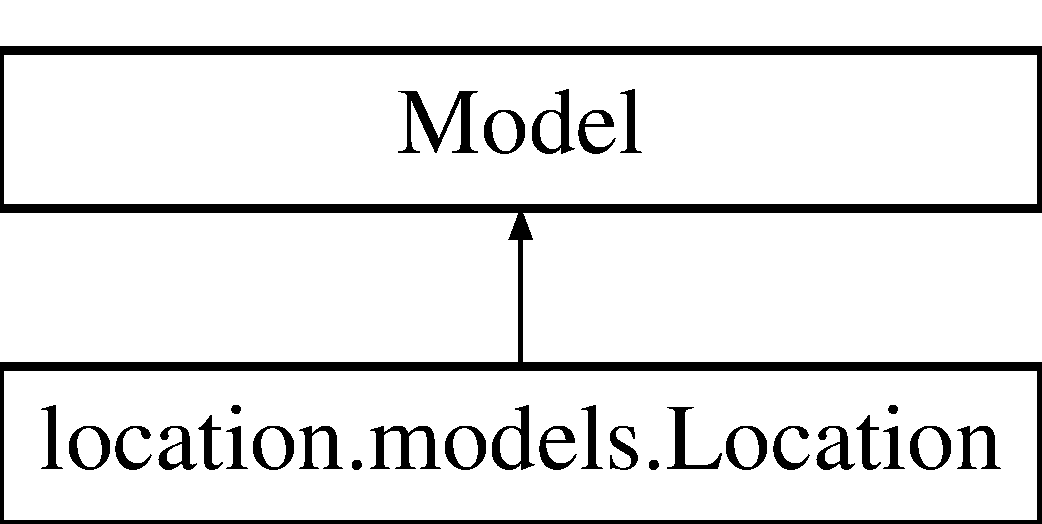
\includegraphics[height=2.000000cm]{classlocation_1_1models_1_1Location}
\end{center}
\end{figure}
\subsection*{Public Member Functions}
\begin{DoxyCompactItemize}
\item 
\hypertarget{classlocation_1_1models_1_1Location_a4ec1d4870386917e6653b7c54d43605e}{def {\bfseries \-\_\-\-\_\-str\-\_\-\-\_\-}}\label{classlocation_1_1models_1_1Location_a4ec1d4870386917e6653b7c54d43605e}

\end{DoxyCompactItemize}
\subsection*{Static Public Attributes}
\begin{DoxyCompactItemize}
\item 
\hypertarget{classlocation_1_1models_1_1Location_a762901546b3ee3d286a82610e54477fc}{tuple {\bfseries x} = models.\-Float\-Field(default=0)}\label{classlocation_1_1models_1_1Location_a762901546b3ee3d286a82610e54477fc}

\item 
\hypertarget{classlocation_1_1models_1_1Location_a0076656a7475178556120670536e449a}{tuple {\bfseries y} = models.\-Float\-Field(default=0)}\label{classlocation_1_1models_1_1Location_a0076656a7475178556120670536e449a}

\item 
\hypertarget{classlocation_1_1models_1_1Location_a33b4be7eef0bcaacc8bcdb3c1d934074}{tuple {\bfseries z} = models.\-Float\-Field(default=0)}\label{classlocation_1_1models_1_1Location_a33b4be7eef0bcaacc8bcdb3c1d934074}

\end{DoxyCompactItemize}


\subsection{Detailed Description}
Class linked to the \hyperlink{classlocation_1_1models_1_1Location}{Location} table in the database. 

The documentation for this class was generated from the following file\-:\begin{DoxyCompactItemize}
\item 
server/location/models.\-py\end{DoxyCompactItemize}

\hypertarget{classcom_1_1example_1_1fabien_1_1lo53__project_1_1MainActivity}{\section{com.\-example.\-fabien.\-lo53\-\_\-project.\-Main\-Activity Class Reference}
\label{classcom_1_1example_1_1fabien_1_1lo53__project_1_1MainActivity}\index{com.\-example.\-fabien.\-lo53\-\_\-project.\-Main\-Activity@{com.\-example.\-fabien.\-lo53\-\_\-project.\-Main\-Activity}}
}
Inheritance diagram for com.\-example.\-fabien.\-lo53\-\_\-project.\-Main\-Activity\-:\begin{figure}[H]
\begin{center}
\leavevmode
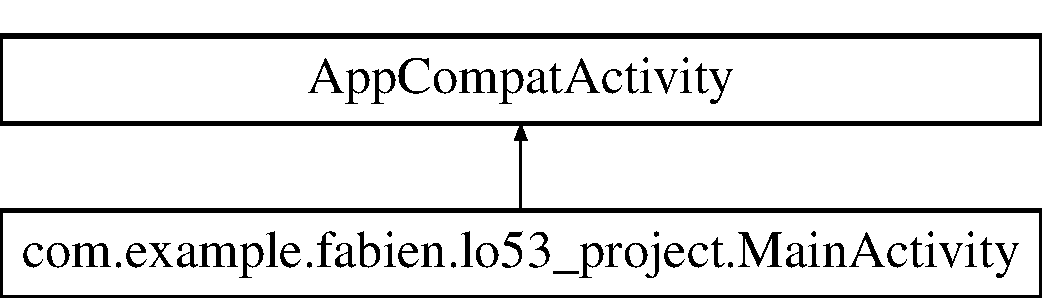
\includegraphics[height=2.000000cm]{classcom_1_1example_1_1fabien_1_1lo53__project_1_1MainActivity}
\end{center}
\end{figure}
\subsection*{Public Member Functions}
\begin{DoxyCompactItemize}
\item 
boolean \hyperlink{classcom_1_1example_1_1fabien_1_1lo53__project_1_1MainActivity_adff8bc0d7f447c04b51b445b311d3dcd}{on\-Create\-Options\-Menu} (Menu menu)
\item 
boolean \hyperlink{classcom_1_1example_1_1fabien_1_1lo53__project_1_1MainActivity_a28e11fb5c445043c22ffddd3e9207ada}{on\-Options\-Item\-Selected} (Menu\-Item item)
\item 
boolean \hyperlink{classcom_1_1example_1_1fabien_1_1lo53__project_1_1MainActivity_a3c23459190c309b08aa0c185db2676bc}{on\-Touch\-Event} (Motion\-Event event)
\item 
void \hyperlink{classcom_1_1example_1_1fabien_1_1lo53__project_1_1MainActivity_a31118445953585f2d27b1b9b044e4987}{send\-Reset} ()
\item 
void \hyperlink{classcom_1_1example_1_1fabien_1_1lo53__project_1_1MainActivity_a957f36de03d8e07d8e405568d7b8319d}{move\-Cursor} (int x, int y)
\item 
void \hyperlink{classcom_1_1example_1_1fabien_1_1lo53__project_1_1MainActivity_a64efc7252e031de0bd39476bae4c5752}{init\-Mac\-Adresse} ()
\item 
void \hyperlink{classcom_1_1example_1_1fabien_1_1lo53__project_1_1MainActivity_ade905e90c38949e097e34396cbb49ffa}{init\-Dialog\-Step\-Calibration} ()
\item 
void \hyperlink{classcom_1_1example_1_1fabien_1_1lo53__project_1_1MainActivity_a5571fd0a612074cc7af2f3b2dd1ad45e}{on\-Empty\-Dialog\-Response} ()
\item 
void \hyperlink{classcom_1_1example_1_1fabien_1_1lo53__project_1_1MainActivity_a9f71f4fb957b11c7e2bbca11533f1ae4}{init\-Calibrate\-Requete} ()
\item 
void \hyperlink{classcom_1_1example_1_1fabien_1_1lo53__project_1_1MainActivity_a657b41f3e170fae1cd6a3fae64c28433}{init\-Refresh\-Requete} ()
\item 
void \hyperlink{classcom_1_1example_1_1fabien_1_1lo53__project_1_1MainActivity_aa9be6a48c39c3612ce969eea85173bb4}{init\-Button} ()
\item 
void \hyperlink{classcom_1_1example_1_1fabien_1_1lo53__project_1_1MainActivity_ac7c0fe459218d9d65c3fd2ec696d88e0}{init\-Cursor} ()
\item 
void \hyperlink{classcom_1_1example_1_1fabien_1_1lo53__project_1_1MainActivity_ac08b9664768c62c86b6fb6fe3c5acb83}{init\-Pixel\-Calibration} ()
\item 
void \hyperlink{classcom_1_1example_1_1fabien_1_1lo53__project_1_1MainActivity_a07572b87e5bb5d6fb795194f414f33b3}{init\-Counter} ()
\end{DoxyCompactItemize}
\subsection*{Protected Member Functions}
\begin{DoxyCompactItemize}
\item 
void \hyperlink{classcom_1_1example_1_1fabien_1_1lo53__project_1_1MainActivity_a1e9059c6c2bcebb6e75b78cb4588b98a}{on\-Create} (Bundle saved\-Instance\-State)
\item 
void \hyperlink{classcom_1_1example_1_1fabien_1_1lo53__project_1_1MainActivity_a339cbc5d541c09e162894c57a8b81616}{on\-Start} ()
\item 
void \hyperlink{classcom_1_1example_1_1fabien_1_1lo53__project_1_1MainActivity_a7f0257fe40603349f15a4b4fdfb31864}{on\-Stop} ()
\end{DoxyCompactItemize}


\subsection{Member Function Documentation}
\hypertarget{classcom_1_1example_1_1fabien_1_1lo53__project_1_1MainActivity_aa9be6a48c39c3612ce969eea85173bb4}{\index{com\-::example\-::fabien\-::lo53\-\_\-project\-::\-Main\-Activity@{com\-::example\-::fabien\-::lo53\-\_\-project\-::\-Main\-Activity}!init\-Button@{init\-Button}}
\index{init\-Button@{init\-Button}!com::example::fabien::lo53_project::MainActivity@{com\-::example\-::fabien\-::lo53\-\_\-project\-::\-Main\-Activity}}
\subsubsection[{init\-Button}]{\setlength{\rightskip}{0pt plus 5cm}void com.\-example.\-fabien.\-lo53\-\_\-project.\-Main\-Activity.\-init\-Button (
\begin{DoxyParamCaption}
{}
\end{DoxyParamCaption}
)\hspace{0.3cm}{\ttfamily [inline]}}}\label{classcom_1_1example_1_1fabien_1_1lo53__project_1_1MainActivity_aa9be6a48c39c3612ce969eea85173bb4}
Methode permettant d'initialiser les différents bouton intégrés à l'application 1\-\_\-\-\_\-\-\_\-valid\-Position utile lors de la calibration pour valider l'origine 2\-\_\-\-\_\-\-\_\-end\-Calibreation utile pour valider la fin de la calibration 3\-\_\-\-\_\-\-\_\-send\-Coord utile pour envoyer les coord de chaque point lors de la calibration \hypertarget{classcom_1_1example_1_1fabien_1_1lo53__project_1_1MainActivity_a9f71f4fb957b11c7e2bbca11533f1ae4}{\index{com\-::example\-::fabien\-::lo53\-\_\-project\-::\-Main\-Activity@{com\-::example\-::fabien\-::lo53\-\_\-project\-::\-Main\-Activity}!init\-Calibrate\-Requete@{init\-Calibrate\-Requete}}
\index{init\-Calibrate\-Requete@{init\-Calibrate\-Requete}!com::example::fabien::lo53_project::MainActivity@{com\-::example\-::fabien\-::lo53\-\_\-project\-::\-Main\-Activity}}
\subsubsection[{init\-Calibrate\-Requete}]{\setlength{\rightskip}{0pt plus 5cm}void com.\-example.\-fabien.\-lo53\-\_\-project.\-Main\-Activity.\-init\-Calibrate\-Requete (
\begin{DoxyParamCaption}
{}
\end{DoxyParamCaption}
)\hspace{0.3cm}{\ttfamily [inline]}}}\label{classcom_1_1example_1_1fabien_1_1lo53__project_1_1MainActivity_a9f71f4fb957b11c7e2bbca11533f1ae4}
Methode qui crée et initialise les requetes J\-S\-O\-N de calibration 1\-\_\-\-\_\-\-\_\-le code a executer lors d'une réponse 2\-\_\-\-\_\-\-\_\-le code a executer lors d'un T\-I\-M\-E\-O\-U\-T \hypertarget{classcom_1_1example_1_1fabien_1_1lo53__project_1_1MainActivity_a07572b87e5bb5d6fb795194f414f33b3}{\index{com\-::example\-::fabien\-::lo53\-\_\-project\-::\-Main\-Activity@{com\-::example\-::fabien\-::lo53\-\_\-project\-::\-Main\-Activity}!init\-Counter@{init\-Counter}}
\index{init\-Counter@{init\-Counter}!com::example::fabien::lo53_project::MainActivity@{com\-::example\-::fabien\-::lo53\-\_\-project\-::\-Main\-Activity}}
\subsubsection[{init\-Counter}]{\setlength{\rightskip}{0pt plus 5cm}void com.\-example.\-fabien.\-lo53\-\_\-project.\-Main\-Activity.\-init\-Counter (
\begin{DoxyParamCaption}
{}
\end{DoxyParamCaption}
)\hspace{0.3cm}{\ttfamily [inline]}}}\label{classcom_1_1example_1_1fabien_1_1lo53__project_1_1MainActivity_a07572b87e5bb5d6fb795194f414f33b3}
Methode permettant d'initialiser le timer du programme Ce timer permet l'envoie tous les 500 ms des requetes U\-R\-L suivant le mode actif (calibration ou Find me ). Ce timer est lancer et areter dans le reste du code suivant l'execution \hypertarget{classcom_1_1example_1_1fabien_1_1lo53__project_1_1MainActivity_ac7c0fe459218d9d65c3fd2ec696d88e0}{\index{com\-::example\-::fabien\-::lo53\-\_\-project\-::\-Main\-Activity@{com\-::example\-::fabien\-::lo53\-\_\-project\-::\-Main\-Activity}!init\-Cursor@{init\-Cursor}}
\index{init\-Cursor@{init\-Cursor}!com::example::fabien::lo53_project::MainActivity@{com\-::example\-::fabien\-::lo53\-\_\-project\-::\-Main\-Activity}}
\subsubsection[{init\-Cursor}]{\setlength{\rightskip}{0pt plus 5cm}void com.\-example.\-fabien.\-lo53\-\_\-project.\-Main\-Activity.\-init\-Cursor (
\begin{DoxyParamCaption}
{}
\end{DoxyParamCaption}
)\hspace{0.3cm}{\ttfamily [inline]}}}\label{classcom_1_1example_1_1fabien_1_1lo53__project_1_1MainActivity_ac7c0fe459218d9d65c3fd2ec696d88e0}
Methode permettant d'initialiser l'image du curseur \hypertarget{classcom_1_1example_1_1fabien_1_1lo53__project_1_1MainActivity_ade905e90c38949e097e34396cbb49ffa}{\index{com\-::example\-::fabien\-::lo53\-\_\-project\-::\-Main\-Activity@{com\-::example\-::fabien\-::lo53\-\_\-project\-::\-Main\-Activity}!init\-Dialog\-Step\-Calibration@{init\-Dialog\-Step\-Calibration}}
\index{init\-Dialog\-Step\-Calibration@{init\-Dialog\-Step\-Calibration}!com::example::fabien::lo53_project::MainActivity@{com\-::example\-::fabien\-::lo53\-\_\-project\-::\-Main\-Activity}}
\subsubsection[{init\-Dialog\-Step\-Calibration}]{\setlength{\rightskip}{0pt plus 5cm}void com.\-example.\-fabien.\-lo53\-\_\-project.\-Main\-Activity.\-init\-Dialog\-Step\-Calibration (
\begin{DoxyParamCaption}
{}
\end{DoxyParamCaption}
)\hspace{0.3cm}{\ttfamily [inline]}}}\label{classcom_1_1example_1_1fabien_1_1lo53__project_1_1MainActivity_ade905e90c38949e097e34396cbb49ffa}
Methode permettant d'initialiser le dialogue concernant la demande à l'utilisateur du pas de calibration en metre \hypertarget{classcom_1_1example_1_1fabien_1_1lo53__project_1_1MainActivity_a64efc7252e031de0bd39476bae4c5752}{\index{com\-::example\-::fabien\-::lo53\-\_\-project\-::\-Main\-Activity@{com\-::example\-::fabien\-::lo53\-\_\-project\-::\-Main\-Activity}!init\-Mac\-Adresse@{init\-Mac\-Adresse}}
\index{init\-Mac\-Adresse@{init\-Mac\-Adresse}!com::example::fabien::lo53_project::MainActivity@{com\-::example\-::fabien\-::lo53\-\_\-project\-::\-Main\-Activity}}
\subsubsection[{init\-Mac\-Adresse}]{\setlength{\rightskip}{0pt plus 5cm}void com.\-example.\-fabien.\-lo53\-\_\-project.\-Main\-Activity.\-init\-Mac\-Adresse (
\begin{DoxyParamCaption}
{}
\end{DoxyParamCaption}
)\hspace{0.3cm}{\ttfamily [inline]}}}\label{classcom_1_1example_1_1fabien_1_1lo53__project_1_1MainActivity_a64efc7252e031de0bd39476bae4c5752}
Methode permettant de récuperer l'adresse M\-A\-C propre au mobile et d'implementer cette derniere dans les U\-R\-L a envoyer \hypertarget{classcom_1_1example_1_1fabien_1_1lo53__project_1_1MainActivity_ac08b9664768c62c86b6fb6fe3c5acb83}{\index{com\-::example\-::fabien\-::lo53\-\_\-project\-::\-Main\-Activity@{com\-::example\-::fabien\-::lo53\-\_\-project\-::\-Main\-Activity}!init\-Pixel\-Calibration@{init\-Pixel\-Calibration}}
\index{init\-Pixel\-Calibration@{init\-Pixel\-Calibration}!com::example::fabien::lo53_project::MainActivity@{com\-::example\-::fabien\-::lo53\-\_\-project\-::\-Main\-Activity}}
\subsubsection[{init\-Pixel\-Calibration}]{\setlength{\rightskip}{0pt plus 5cm}void com.\-example.\-fabien.\-lo53\-\_\-project.\-Main\-Activity.\-init\-Pixel\-Calibration (
\begin{DoxyParamCaption}
{}
\end{DoxyParamCaption}
)\hspace{0.3cm}{\ttfamily [inline]}}}\label{classcom_1_1example_1_1fabien_1_1lo53__project_1_1MainActivity_ac08b9664768c62c86b6fb6fe3c5acb83}
Methode ayant pour but d'autoriser la calibration de la position d'origine par l'utilisateur via la position du doigt du l'écran (methode on\-Touch surchargée) \hypertarget{classcom_1_1example_1_1fabien_1_1lo53__project_1_1MainActivity_a657b41f3e170fae1cd6a3fae64c28433}{\index{com\-::example\-::fabien\-::lo53\-\_\-project\-::\-Main\-Activity@{com\-::example\-::fabien\-::lo53\-\_\-project\-::\-Main\-Activity}!init\-Refresh\-Requete@{init\-Refresh\-Requete}}
\index{init\-Refresh\-Requete@{init\-Refresh\-Requete}!com::example::fabien::lo53_project::MainActivity@{com\-::example\-::fabien\-::lo53\-\_\-project\-::\-Main\-Activity}}
\subsubsection[{init\-Refresh\-Requete}]{\setlength{\rightskip}{0pt plus 5cm}void com.\-example.\-fabien.\-lo53\-\_\-project.\-Main\-Activity.\-init\-Refresh\-Requete (
\begin{DoxyParamCaption}
{}
\end{DoxyParamCaption}
)\hspace{0.3cm}{\ttfamily [inline]}}}\label{classcom_1_1example_1_1fabien_1_1lo53__project_1_1MainActivity_a657b41f3e170fae1cd6a3fae64c28433}
Methode qui crée et initialise les requetes J\-S\-O\-N de F\-I\-N\-D M\-E 1\-\_\-\-\_\-\-\_\-le code a executer lors d'une réponse 2\-\_\-\-\_\-\-\_\-le code a executer lors d'un T\-I\-M\-E\-O\-U\-T \hypertarget{classcom_1_1example_1_1fabien_1_1lo53__project_1_1MainActivity_a957f36de03d8e07d8e405568d7b8319d}{\index{com\-::example\-::fabien\-::lo53\-\_\-project\-::\-Main\-Activity@{com\-::example\-::fabien\-::lo53\-\_\-project\-::\-Main\-Activity}!move\-Cursor@{move\-Cursor}}
\index{move\-Cursor@{move\-Cursor}!com::example::fabien::lo53_project::MainActivity@{com\-::example\-::fabien\-::lo53\-\_\-project\-::\-Main\-Activity}}
\subsubsection[{move\-Cursor}]{\setlength{\rightskip}{0pt plus 5cm}void com.\-example.\-fabien.\-lo53\-\_\-project.\-Main\-Activity.\-move\-Cursor (
\begin{DoxyParamCaption}
\item[{int}]{x, }
\item[{int}]{y}
\end{DoxyParamCaption}
)\hspace{0.3cm}{\ttfamily [inline]}}}\label{classcom_1_1example_1_1fabien_1_1lo53__project_1_1MainActivity_a957f36de03d8e07d8e405568d7b8319d}
Methode permettant de deplacer le curseur suivant ses coordonnées \hypertarget{classcom_1_1example_1_1fabien_1_1lo53__project_1_1MainActivity_a1e9059c6c2bcebb6e75b78cb4588b98a}{\index{com\-::example\-::fabien\-::lo53\-\_\-project\-::\-Main\-Activity@{com\-::example\-::fabien\-::lo53\-\_\-project\-::\-Main\-Activity}!on\-Create@{on\-Create}}
\index{on\-Create@{on\-Create}!com::example::fabien::lo53_project::MainActivity@{com\-::example\-::fabien\-::lo53\-\_\-project\-::\-Main\-Activity}}
\subsubsection[{on\-Create}]{\setlength{\rightskip}{0pt plus 5cm}void com.\-example.\-fabien.\-lo53\-\_\-project.\-Main\-Activity.\-on\-Create (
\begin{DoxyParamCaption}
\item[{Bundle}]{saved\-Instance\-State}
\end{DoxyParamCaption}
)\hspace{0.3cm}{\ttfamily [inline]}, {\ttfamily [protected]}}}\label{classcom_1_1example_1_1fabien_1_1lo53__project_1_1MainActivity_a1e9059c6c2bcebb6e75b78cb4588b98a}
Methode qui se déclanche automatiquement au lancement de l'application Elle représente la création de notre activité. = Lancement de toute les initialisations nécessaires au programme et activation du timer qui cadence les envoies U\-R\-L (mode de démarage = Find Me) \hypertarget{classcom_1_1example_1_1fabien_1_1lo53__project_1_1MainActivity_adff8bc0d7f447c04b51b445b311d3dcd}{\index{com\-::example\-::fabien\-::lo53\-\_\-project\-::\-Main\-Activity@{com\-::example\-::fabien\-::lo53\-\_\-project\-::\-Main\-Activity}!on\-Create\-Options\-Menu@{on\-Create\-Options\-Menu}}
\index{on\-Create\-Options\-Menu@{on\-Create\-Options\-Menu}!com::example::fabien::lo53_project::MainActivity@{com\-::example\-::fabien\-::lo53\-\_\-project\-::\-Main\-Activity}}
\subsubsection[{on\-Create\-Options\-Menu}]{\setlength{\rightskip}{0pt plus 5cm}boolean com.\-example.\-fabien.\-lo53\-\_\-project.\-Main\-Activity.\-on\-Create\-Options\-Menu (
\begin{DoxyParamCaption}
\item[{Menu}]{menu}
\end{DoxyParamCaption}
)\hspace{0.3cm}{\ttfamily [inline]}}}\label{classcom_1_1example_1_1fabien_1_1lo53__project_1_1MainActivity_adff8bc0d7f447c04b51b445b311d3dcd}
Methode permettant d'initialiser le menu option (avec l'option nouvelle calibration decrit en X\-M\-L) \hypertarget{classcom_1_1example_1_1fabien_1_1lo53__project_1_1MainActivity_a5571fd0a612074cc7af2f3b2dd1ad45e}{\index{com\-::example\-::fabien\-::lo53\-\_\-project\-::\-Main\-Activity@{com\-::example\-::fabien\-::lo53\-\_\-project\-::\-Main\-Activity}!on\-Empty\-Dialog\-Response@{on\-Empty\-Dialog\-Response}}
\index{on\-Empty\-Dialog\-Response@{on\-Empty\-Dialog\-Response}!com::example::fabien::lo53_project::MainActivity@{com\-::example\-::fabien\-::lo53\-\_\-project\-::\-Main\-Activity}}
\subsubsection[{on\-Empty\-Dialog\-Response}]{\setlength{\rightskip}{0pt plus 5cm}void com.\-example.\-fabien.\-lo53\-\_\-project.\-Main\-Activity.\-on\-Empty\-Dialog\-Response (
\begin{DoxyParamCaption}
{}
\end{DoxyParamCaption}
)\hspace{0.3cm}{\ttfamily [inline]}}}\label{classcom_1_1example_1_1fabien_1_1lo53__project_1_1MainActivity_a5571fd0a612074cc7af2f3b2dd1ad45e}
Methode permettant de relancer le dialogue ci-\/dessus en cas d'un saisie invalide (Pour eviter de faire planter l'application) \hypertarget{classcom_1_1example_1_1fabien_1_1lo53__project_1_1MainActivity_a28e11fb5c445043c22ffddd3e9207ada}{\index{com\-::example\-::fabien\-::lo53\-\_\-project\-::\-Main\-Activity@{com\-::example\-::fabien\-::lo53\-\_\-project\-::\-Main\-Activity}!on\-Options\-Item\-Selected@{on\-Options\-Item\-Selected}}
\index{on\-Options\-Item\-Selected@{on\-Options\-Item\-Selected}!com::example::fabien::lo53_project::MainActivity@{com\-::example\-::fabien\-::lo53\-\_\-project\-::\-Main\-Activity}}
\subsubsection[{on\-Options\-Item\-Selected}]{\setlength{\rightskip}{0pt plus 5cm}boolean com.\-example.\-fabien.\-lo53\-\_\-project.\-Main\-Activity.\-on\-Options\-Item\-Selected (
\begin{DoxyParamCaption}
\item[{Menu\-Item}]{item}
\end{DoxyParamCaption}
)\hspace{0.3cm}{\ttfamily [inline]}}}\label{classcom_1_1example_1_1fabien_1_1lo53__project_1_1MainActivity_a28e11fb5c445043c22ffddd3e9207ada}
Méthode s'activement automatique lors de la selection d'une option dans le menu Dans notre cas la seule option disponible est \char`\"{}nouvelle calibration\char`\"{} \hypertarget{classcom_1_1example_1_1fabien_1_1lo53__project_1_1MainActivity_a339cbc5d541c09e162894c57a8b81616}{\index{com\-::example\-::fabien\-::lo53\-\_\-project\-::\-Main\-Activity@{com\-::example\-::fabien\-::lo53\-\_\-project\-::\-Main\-Activity}!on\-Start@{on\-Start}}
\index{on\-Start@{on\-Start}!com::example::fabien::lo53_project::MainActivity@{com\-::example\-::fabien\-::lo53\-\_\-project\-::\-Main\-Activity}}
\subsubsection[{on\-Start}]{\setlength{\rightskip}{0pt plus 5cm}void com.\-example.\-fabien.\-lo53\-\_\-project.\-Main\-Activity.\-on\-Start (
\begin{DoxyParamCaption}
{}
\end{DoxyParamCaption}
)\hspace{0.3cm}{\ttfamily [inline]}, {\ttfamily [protected]}}}\label{classcom_1_1example_1_1fabien_1_1lo53__project_1_1MainActivity_a339cbc5d541c09e162894c57a8b81616}
Methode qui se déclanche automatiquement lorsque notre activité prend le focus de l'écran. Se déclanche après le on\-Create lors du démarage de l'application. Cette méthode nous sert à récupere la dimenssion actuelle de l'activité (suivant les telephone) et de lancer le calcul du ratio suivant ces informations Le code implémenté ici ne fonctionne pas dans le on\-Create raison pour laquelle nous devons surcharger cette méthode \hypertarget{classcom_1_1example_1_1fabien_1_1lo53__project_1_1MainActivity_a7f0257fe40603349f15a4b4fdfb31864}{\index{com\-::example\-::fabien\-::lo53\-\_\-project\-::\-Main\-Activity@{com\-::example\-::fabien\-::lo53\-\_\-project\-::\-Main\-Activity}!on\-Stop@{on\-Stop}}
\index{on\-Stop@{on\-Stop}!com::example::fabien::lo53_project::MainActivity@{com\-::example\-::fabien\-::lo53\-\_\-project\-::\-Main\-Activity}}
\subsubsection[{on\-Stop}]{\setlength{\rightskip}{0pt plus 5cm}void com.\-example.\-fabien.\-lo53\-\_\-project.\-Main\-Activity.\-on\-Stop (
\begin{DoxyParamCaption}
{}
\end{DoxyParamCaption}
)\hspace{0.3cm}{\ttfamily [inline]}, {\ttfamily [protected]}}}\label{classcom_1_1example_1_1fabien_1_1lo53__project_1_1MainActivity_a7f0257fe40603349f15a4b4fdfb31864}
Methode appelé lors de la perte du focus par l'application \hypertarget{classcom_1_1example_1_1fabien_1_1lo53__project_1_1MainActivity_a3c23459190c309b08aa0c185db2676bc}{\index{com\-::example\-::fabien\-::lo53\-\_\-project\-::\-Main\-Activity@{com\-::example\-::fabien\-::lo53\-\_\-project\-::\-Main\-Activity}!on\-Touch\-Event@{on\-Touch\-Event}}
\index{on\-Touch\-Event@{on\-Touch\-Event}!com::example::fabien::lo53_project::MainActivity@{com\-::example\-::fabien\-::lo53\-\_\-project\-::\-Main\-Activity}}
\subsubsection[{on\-Touch\-Event}]{\setlength{\rightskip}{0pt plus 5cm}boolean com.\-example.\-fabien.\-lo53\-\_\-project.\-Main\-Activity.\-on\-Touch\-Event (
\begin{DoxyParamCaption}
\item[{Motion\-Event}]{event}
\end{DoxyParamCaption}
)\hspace{0.3cm}{\ttfamily [inline]}}}\label{classcom_1_1example_1_1fabien_1_1lo53__project_1_1MainActivity_a3c23459190c309b08aa0c185db2676bc}
Methode qui se déclanche automatiquement lorsque l'utilisateur intéragie avec l'écran. Mais elle n'est prise en compte que lorsque l'utilisateur doit initialiser la position d'origine via l'écran (au début de chaque calibration) \hypertarget{classcom_1_1example_1_1fabien_1_1lo53__project_1_1MainActivity_a31118445953585f2d27b1b9b044e4987}{\index{com\-::example\-::fabien\-::lo53\-\_\-project\-::\-Main\-Activity@{com\-::example\-::fabien\-::lo53\-\_\-project\-::\-Main\-Activity}!send\-Reset@{send\-Reset}}
\index{send\-Reset@{send\-Reset}!com::example::fabien::lo53_project::MainActivity@{com\-::example\-::fabien\-::lo53\-\_\-project\-::\-Main\-Activity}}
\subsubsection[{send\-Reset}]{\setlength{\rightskip}{0pt plus 5cm}void com.\-example.\-fabien.\-lo53\-\_\-project.\-Main\-Activity.\-send\-Reset (
\begin{DoxyParamCaption}
{}
\end{DoxyParamCaption}
)\hspace{0.3cm}{\ttfamily [inline]}}}\label{classcom_1_1example_1_1fabien_1_1lo53__project_1_1MainActivity_a31118445953585f2d27b1b9b044e4987}
Methode permettant l'envoie d'une requête H\-T\-T\-P Reset 

The documentation for this class was generated from the following file\-:\begin{DoxyCompactItemize}
\item 
appli/app/src/main/java/com/example/fabien/lo53\-\_\-project/Main\-Activity.\-java\end{DoxyCompactItemize}

\hypertarget{classlocation_1_1models_1_1Measurement}{\section{location.\-models.\-Measurement Class Reference}
\label{classlocation_1_1models_1_1Measurement}\index{location.\-models.\-Measurement@{location.\-models.\-Measurement}}
}


Class linked to the Measurment table in the database.  


Inheritance diagram for location.\-models.\-Measurement\-:\begin{figure}[H]
\begin{center}
\leavevmode
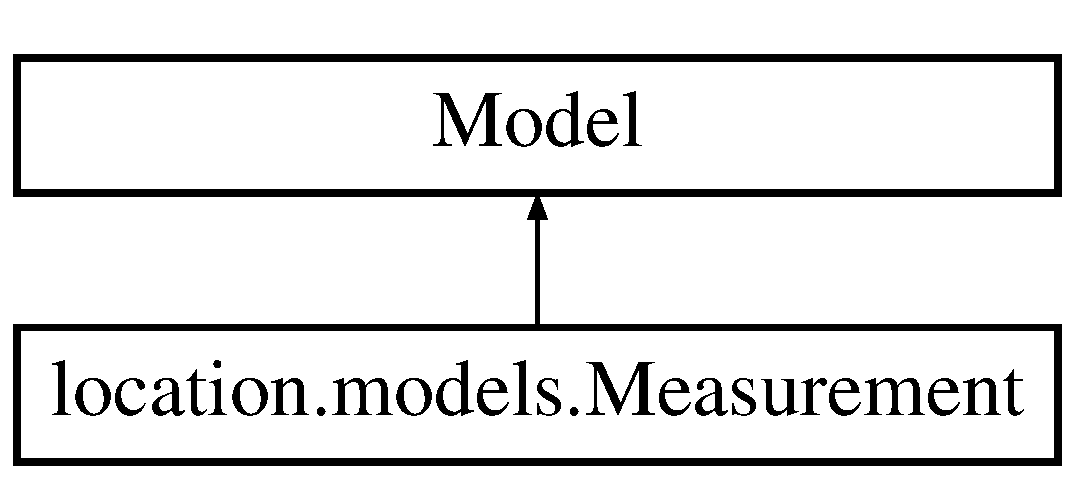
\includegraphics[height=2.000000cm]{classlocation_1_1models_1_1Measurement}
\end{center}
\end{figure}
\subsection*{Static Public Member Functions}
\begin{DoxyCompactItemize}
\item 
def \hyperlink{classlocation_1_1models_1_1Measurement_a763d73da289bc8117bdbded89c80a12f}{ss\-\_\-average}
\begin{DoxyCompactList}\small\item\em Compute the average of all the measurments for a given device and a given access-\/point. \end{DoxyCompactList}\end{DoxyCompactItemize}
\subsection*{Static Public Attributes}
\begin{DoxyCompactItemize}
\item 
\hypertarget{classlocation_1_1models_1_1Measurement_a6e9937292430758f3c99f0a8ee641ecc}{tuple {\bfseries ap\-\_\-id} = models.\-Integer\-Field(default=0)}\label{classlocation_1_1models_1_1Measurement_a6e9937292430758f3c99f0a8ee641ecc}

\item 
\hypertarget{classlocation_1_1models_1_1Measurement_a566d8eb7ccdca69a0bcfb600572dcb2f}{tuple {\bfseries dv\-\_\-id} = models.\-Foreign\-Key(\hyperlink{classlocation_1_1models_1_1Device}{Device}, on\-\_\-delete=models.\-C\-A\-S\-C\-A\-D\-E)}\label{classlocation_1_1models_1_1Measurement_a566d8eb7ccdca69a0bcfb600572dcb2f}

\item 
\hypertarget{classlocation_1_1models_1_1Measurement_a51b46b31cf97b48211bf482e24c05884}{tuple {\bfseries ss\-\_\-value} = models.\-Float\-Field(default=0)}\label{classlocation_1_1models_1_1Measurement_a51b46b31cf97b48211bf482e24c05884}

\end{DoxyCompactItemize}


\subsection{Detailed Description}
Class linked to the Measurment table in the database. 

\subsection{Member Function Documentation}
\hypertarget{classlocation_1_1models_1_1Measurement_a763d73da289bc8117bdbded89c80a12f}{\index{location\-::models\-::\-Measurement@{location\-::models\-::\-Measurement}!ss\-\_\-average@{ss\-\_\-average}}
\index{ss\-\_\-average@{ss\-\_\-average}!location::models::Measurement@{location\-::models\-::\-Measurement}}
\subsubsection[{ss\-\_\-average}]{\setlength{\rightskip}{0pt plus 5cm}def location.\-models.\-Measurement.\-ss\-\_\-average (
\begin{DoxyParamCaption}
\item[{}]{ap\-\_\-id, }
\item[{}]{dv\-\_\-id}
\end{DoxyParamCaption}
)\hspace{0.3cm}{\ttfamily [static]}}}\label{classlocation_1_1models_1_1Measurement_a763d73da289bc8117bdbded89c80a12f}


Compute the average of all the measurments for a given device and a given access-\/point. 


\begin{DoxyParams}{Parameters}
{\em ap\-\_\-id} & Identifier of the access point \\
\hline
{\em dv\-\_\-id} & Identifier of the device \\
\hline
\end{DoxyParams}


The documentation for this class was generated from the following file\-:\begin{DoxyCompactItemize}
\item 
server/location/models.\-py\end{DoxyCompactItemize}

\hypertarget{classcom_1_1example_1_1fabien_1_1lo53__project_1_1MySingleton}{\section{com.\-example.\-fabien.\-lo53\-\_\-project.\-My\-Singleton Class Reference}
\label{classcom_1_1example_1_1fabien_1_1lo53__project_1_1MySingleton}\index{com.\-example.\-fabien.\-lo53\-\_\-project.\-My\-Singleton@{com.\-example.\-fabien.\-lo53\-\_\-project.\-My\-Singleton}}
}
\subsection*{Public Member Functions}
\begin{DoxyCompactItemize}
\item 
\hypertarget{classcom_1_1example_1_1fabien_1_1lo53__project_1_1MySingleton_a776e1f11fb39ca20e4a73a49e41eec1b}{Request\-Queue {\bfseries get\-Request\-Queue} ()}\label{classcom_1_1example_1_1fabien_1_1lo53__project_1_1MySingleton_a776e1f11fb39ca20e4a73a49e41eec1b}

\end{DoxyCompactItemize}
\subsection*{Static Public Member Functions}
\begin{DoxyCompactItemize}
\item 
\hypertarget{classcom_1_1example_1_1fabien_1_1lo53__project_1_1MySingleton_acb6746adad651c17ef1b1c56d715c576}{static synchronized \hyperlink{classcom_1_1example_1_1fabien_1_1lo53__project_1_1MySingleton}{My\-Singleton} {\bfseries get\-Instance} (Context context)}\label{classcom_1_1example_1_1fabien_1_1lo53__project_1_1MySingleton_acb6746adad651c17ef1b1c56d715c576}

\end{DoxyCompactItemize}


\subsection{Detailed Description}
Created by Fabien on 07/06/2016. 

The documentation for this class was generated from the following file\-:\begin{DoxyCompactItemize}
\item 
appli/app/src/main/java/com/example/fabien/lo53\-\_\-project/My\-Singleton.\-java\end{DoxyCompactItemize}

\hypertarget{structradiotap__align__size}{\section{radiotap\-\_\-align\-\_\-size Struct Reference}
\label{structradiotap__align__size}\index{radiotap\-\_\-align\-\_\-size@{radiotap\-\_\-align\-\_\-size}}
}


Alignements and size of the radiotap header field From radiotap.\-c here \href{http://goo.gl/8pk0R9}{\tt http\-://goo.\-gl/8pk0\-R9}.  




{\ttfamily \#include $<$pcap-\/thread.\-h$>$}

\subsection*{Public Attributes}
\begin{DoxyCompactItemize}
\item 
\hypertarget{structradiotap__align__size_a3f6034228a4875b0356c9cc9a668f3b7}{uint8\-\_\-t {\bfseries align}}\label{structradiotap__align__size_a3f6034228a4875b0356c9cc9a668f3b7}

\item 
\hypertarget{structradiotap__align__size_a38af123515c7a6f56f0574caaaff050d}{uint8\-\_\-t {\bfseries size}}\label{structradiotap__align__size_a38af123515c7a6f56f0574caaaff050d}

\end{DoxyCompactItemize}


\subsection{Detailed Description}
Alignements and size of the radiotap header field From radiotap.\-c here \href{http://goo.gl/8pk0R9}{\tt http\-://goo.\-gl/8pk0\-R9}. 

Alignements and size of the radiotap header field. 

The documentation for this struct was generated from the following file\-:\begin{DoxyCompactItemize}
\item 
access-\/point/\hyperlink{pcap-thread_8h}{pcap-\/thread.\-h}\end{DoxyCompactItemize}

\chapter{File Documentation}
\hypertarget{app_8c}{\section{access-\/point/app.c File Reference}
\label{app_8c}\index{access-\/point/app.\-c@{access-\/point/app.\-c}}
}


File that contains the main of the application.  


{\ttfamily \#include $<$stdio.\-h$>$}\\*
{\ttfamily \#include $<$stdlib.\-h$>$}\\*
{\ttfamily \#include $<$pcap.\-h$>$}\\*
{\ttfamily \#include \char`\"{}mac.\-h\char`\"{}}\\*
{\ttfamily \#include \char`\"{}pcap-\/thread.\-h\char`\"{}}\\*
{\ttfamily \#include \char`\"{}http.\-h\char`\"{}}\\*
\subsection*{Functions}
\begin{DoxyCompactItemize}
\item 
int \hyperlink{app_8c_a840291bc02cba5474a4cb46a9b9566fe}{main} (void)
\begin{DoxyCompactList}\small\item\em Entrance of the program. \end{DoxyCompactList}\end{DoxyCompactItemize}


\subsection{Detailed Description}
File that contains the main of the application. \begin{DoxyAuthor}{Author}
vmerat 
\end{DoxyAuthor}
\begin{DoxyVersion}{Version}
0.\-1 
\end{DoxyVersion}
\begin{DoxyDate}{Date}
16/06/16 
\end{DoxyDate}


\subsection{Function Documentation}
\hypertarget{app_8c_a840291bc02cba5474a4cb46a9b9566fe}{\index{app.\-c@{app.\-c}!main@{main}}
\index{main@{main}!app.c@{app.\-c}}
\subsubsection[{main}]{\setlength{\rightskip}{0pt plus 5cm}int main (
\begin{DoxyParamCaption}
\item[{void}]{}
\end{DoxyParamCaption}
)}}\label{app_8c_a840291bc02cba5474a4cb46a9b9566fe}


Entrance of the program. 

\begin{DoxyReturn}{Returns}
an int corresponding to the success of the function or not 
\end{DoxyReturn}

\hypertarget{http_8c}{\section{access-\/point/http.c File Reference}
\label{http_8c}\index{access-\/point/http.\-c@{access-\/point/http.\-c}}
}


H\-T\-T\-P Functions.  


{\ttfamily \#include \char`\"{}http.\-h\char`\"{}}\\*
\subsection*{Functions}
\begin{DoxyCompactItemize}
\item 
void \hyperlink{http_8c_a5a7fd6804526d002c56d864853f4695e}{error} (const char $\ast$msg, int $\ast$success, int sockfd)
\begin{DoxyCompactList}\small\item\em Print the message on the screen, close the socket and update the success value. \end{DoxyCompactList}\item 
char $\ast$ \hyperlink{http_8c_a5b7de03522850319b21022e762cadef0}{http\-\_\-request} (char $\ast$host, char $\ast$message, int $\ast$success)
\begin{DoxyCompactList}\small\item\em Send an http request to the host and the message in parameter. \end{DoxyCompactList}\item 
void \hyperlink{http_8c_a947214d1e90f2e5474ca4bf78db7db72}{send\-\_\-rssi\-\_\-to\-\_\-server} (int rssi, char $\ast$mac\-\_\-string)
\begin{DoxyCompactList}\small\item\em Send to the server the rssi value associated with the mac address. \end{DoxyCompactList}\end{DoxyCompactItemize}


\subsection{Detailed Description}
H\-T\-T\-P Functions. \begin{DoxyAuthor}{Author}
vmerat 
\end{DoxyAuthor}
\begin{DoxyVersion}{Version}
0.\-1 
\end{DoxyVersion}
\begin{DoxyDate}{Date}
16/06/16 H\-T\-T\-P Functions to sends request using this protocol 
\end{DoxyDate}


\subsection{Function Documentation}
\hypertarget{http_8c_a5a7fd6804526d002c56d864853f4695e}{\index{http.\-c@{http.\-c}!error@{error}}
\index{error@{error}!http.c@{http.\-c}}
\subsubsection[{error}]{\setlength{\rightskip}{0pt plus 5cm}void error (
\begin{DoxyParamCaption}
\item[{const char $\ast$}]{msg, }
\item[{int $\ast$}]{success, }
\item[{int}]{sockfd}
\end{DoxyParamCaption}
)}}\label{http_8c_a5a7fd6804526d002c56d864853f4695e}


Print the message on the screen, close the socket and update the success value. 

\begin{DoxyReturn}{Returns}

\end{DoxyReturn}

\begin{DoxyParams}{Parameters}
{\em msg} & an already allocated char buffer \\
\hline
{\em success} & an already allocated int \\
\hline
{\em sockfd} & corresponding to the socket we need to close \\
\hline
\end{DoxyParams}
\hypertarget{http_8c_a5b7de03522850319b21022e762cadef0}{\index{http.\-c@{http.\-c}!http\-\_\-request@{http\-\_\-request}}
\index{http\-\_\-request@{http\-\_\-request}!http.c@{http.\-c}}
\subsubsection[{http\-\_\-request}]{\setlength{\rightskip}{0pt plus 5cm}char $\ast$ http\-\_\-request (
\begin{DoxyParamCaption}
\item[{char $\ast$}]{host, }
\item[{char $\ast$}]{message, }
\item[{int $\ast$}]{success}
\end{DoxyParamCaption}
)}}\label{http_8c_a5b7de03522850319b21022e762cadef0}


Send an http request to the host and the message in parameter. 

\begin{DoxyReturn}{Returns}
response an already allocated char buffer 
\end{DoxyReturn}

\begin{DoxyParams}{Parameters}
{\em host} & an already allocated char buffer \\
\hline
{\em message} & an already allocated char buffer \\
\hline
{\em success} & which will be set at -\/1 if an error occured \\
\hline
\end{DoxyParams}
\hypertarget{http_8c_a947214d1e90f2e5474ca4bf78db7db72}{\index{http.\-c@{http.\-c}!send\-\_\-rssi\-\_\-to\-\_\-server@{send\-\_\-rssi\-\_\-to\-\_\-server}}
\index{send\-\_\-rssi\-\_\-to\-\_\-server@{send\-\_\-rssi\-\_\-to\-\_\-server}!http.c@{http.\-c}}
\subsubsection[{send\-\_\-rssi\-\_\-to\-\_\-server}]{\setlength{\rightskip}{0pt plus 5cm}void send\-\_\-rssi\-\_\-to\-\_\-server (
\begin{DoxyParamCaption}
\item[{int}]{rssi, }
\item[{char $\ast$}]{mac\-\_\-string}
\end{DoxyParamCaption}
)}}\label{http_8c_a947214d1e90f2e5474ca4bf78db7db72}


Send to the server the rssi value associated with the mac address. 

\begin{DoxyReturn}{Returns}

\end{DoxyReturn}

\begin{DoxyParams}{Parameters}
{\em rssi} & an int corresponding to the rssi value \\
\hline
{\em mac\-\_\-string} & an already allocated char buffer \\
\hline
\end{DoxyParams}

\hypertarget{http_8h}{\section{access-\/point/http.h File Reference}
\label{http_8h}\index{access-\/point/http.\-h@{access-\/point/http.\-h}}
}


H\-T\-T\-P Functions.  


{\ttfamily \#include $<$stdio.\-h$>$}\\*
{\ttfamily \#include $<$stdlib.\-h$>$}\\*
{\ttfamily \#include $<$unistd.\-h$>$}\\*
{\ttfamily \#include $<$string.\-h$>$}\\*
{\ttfamily \#include $<$sys/socket.\-h$>$}\\*
{\ttfamily \#include $<$netinet/in.\-h$>$}\\*
{\ttfamily \#include $<$netdb.\-h$>$}\\*
{\ttfamily \#include \char`\"{}mac.\-h\char`\"{}}\\*
\subsection*{Macros}
\begin{DoxyCompactItemize}
\item 
\hypertarget{http_8h_aeca90e1c1c62b70670514ffc18c9dfd4}{\#define {\bfseries M\-E\-S\-S\-A\-G\-E\-\_\-\-S\-I\-Z\-E}~1024}\label{http_8h_aeca90e1c1c62b70670514ffc18c9dfd4}

\item 
\hypertarget{http_8h_a48c115751f544f6dc2232111ecf30708}{\#define {\bfseries R\-E\-S\-P\-O\-N\-S\-E\-\_\-\-S\-I\-Z\-E}~4096}\label{http_8h_a48c115751f544f6dc2232111ecf30708}

\end{DoxyCompactItemize}
\subsection*{Functions}
\begin{DoxyCompactItemize}
\item 
char $\ast$ \hyperlink{http_8h_af9d7b3062e02587caeaa3ca144561c49}{http\-\_\-request} (char $\ast$host, char $\ast$message, int $\ast$success)
\begin{DoxyCompactList}\small\item\em Send an http request to the host and the message in parameter. \end{DoxyCompactList}\item 
void \hyperlink{http_8h_a5a7fd6804526d002c56d864853f4695e}{error} (const char $\ast$msg, int $\ast$success, int sockfd)
\begin{DoxyCompactList}\small\item\em Print the message on the screen, close the socket and update the success value. \end{DoxyCompactList}\item 
void \hyperlink{http_8h_a947214d1e90f2e5474ca4bf78db7db72}{send\-\_\-rssi\-\_\-to\-\_\-server} (int rssi, char $\ast$mac\-\_\-string)
\begin{DoxyCompactList}\small\item\em Send to the server the rssi value associated with the mac address. \end{DoxyCompactList}\end{DoxyCompactItemize}


\subsection{Detailed Description}
H\-T\-T\-P Functions. \begin{DoxyAuthor}{Author}
vmerat 
\end{DoxyAuthor}
\begin{DoxyVersion}{Version}
0.\-1 
\end{DoxyVersion}
\begin{DoxyDate}{Date}
16/06/16 H\-T\-T\-P Functions to sends request using this protocol 
\end{DoxyDate}


\subsection{Function Documentation}
\hypertarget{http_8h_a5a7fd6804526d002c56d864853f4695e}{\index{http.\-h@{http.\-h}!error@{error}}
\index{error@{error}!http.h@{http.\-h}}
\subsubsection[{error}]{\setlength{\rightskip}{0pt plus 5cm}void error (
\begin{DoxyParamCaption}
\item[{const char $\ast$}]{msg, }
\item[{int $\ast$}]{success, }
\item[{int}]{sockfd}
\end{DoxyParamCaption}
)}}\label{http_8h_a5a7fd6804526d002c56d864853f4695e}


Print the message on the screen, close the socket and update the success value. 

\begin{DoxyReturn}{Returns}

\end{DoxyReturn}

\begin{DoxyParams}{Parameters}
{\em msg} & an already allocated char buffer \\
\hline
{\em success} & an already allocated int \\
\hline
{\em sockfd} & corresponding to the socket we need to close \\
\hline
\end{DoxyParams}
\hypertarget{http_8h_af9d7b3062e02587caeaa3ca144561c49}{\index{http.\-h@{http.\-h}!http\-\_\-request@{http\-\_\-request}}
\index{http\-\_\-request@{http\-\_\-request}!http.h@{http.\-h}}
\subsubsection[{http\-\_\-request}]{\setlength{\rightskip}{0pt plus 5cm}char$\ast$ http\-\_\-request (
\begin{DoxyParamCaption}
\item[{char $\ast$}]{host, }
\item[{char $\ast$}]{message, }
\item[{int $\ast$}]{success}
\end{DoxyParamCaption}
)}}\label{http_8h_af9d7b3062e02587caeaa3ca144561c49}


Send an http request to the host and the message in parameter. 

\begin{DoxyReturn}{Returns}
response an already allocated char buffer 
\end{DoxyReturn}

\begin{DoxyParams}{Parameters}
{\em host} & an already allocated char buffer \\
\hline
{\em message} & an already allocated char buffer \\
\hline
{\em success} & which will be set at -\/1 if an error occured \\
\hline
\end{DoxyParams}
\hypertarget{http_8h_a947214d1e90f2e5474ca4bf78db7db72}{\index{http.\-h@{http.\-h}!send\-\_\-rssi\-\_\-to\-\_\-server@{send\-\_\-rssi\-\_\-to\-\_\-server}}
\index{send\-\_\-rssi\-\_\-to\-\_\-server@{send\-\_\-rssi\-\_\-to\-\_\-server}!http.h@{http.\-h}}
\subsubsection[{send\-\_\-rssi\-\_\-to\-\_\-server}]{\setlength{\rightskip}{0pt plus 5cm}void send\-\_\-rssi\-\_\-to\-\_\-server (
\begin{DoxyParamCaption}
\item[{int}]{rssi, }
\item[{char $\ast$}]{mac\-\_\-string}
\end{DoxyParamCaption}
)}}\label{http_8h_a947214d1e90f2e5474ca4bf78db7db72}


Send to the server the rssi value associated with the mac address. 

\begin{DoxyReturn}{Returns}

\end{DoxyReturn}

\begin{DoxyParams}{Parameters}
{\em rssi} & an int corresponding to the rssi value \\
\hline
{\em mac\-\_\-string} & an already allocated char buffer \\
\hline
\end{DoxyParams}

\hypertarget{mac_8c}{\section{access-\/point/mac.c File Reference}
\label{mac_8c}\index{access-\/point/mac.\-c@{access-\/point/mac.\-c}}
}


Usefull M\-A\-C Functions.  


{\ttfamily \#include \char`\"{}mac.\-h\char`\"{}}\\*
\subsection*{Functions}
\begin{DoxyCompactItemize}
\item 
u\-\_\-char $\ast$ \hyperlink{mac_8c_a9847a88fcad0fe8b8491e63f998c6f80}{string\-\_\-to\-\_\-mac} (char $\ast$buf, u\-\_\-char $\ast$byte\-\_\-mac)
\begin{DoxyCompactList}\small\item\em Function string\-\_\-to\-\_\-mac converts a human-\/readable M\-A\-C to its binary counterpart. \end{DoxyCompactList}\item 
char $\ast$ \hyperlink{mac_8c_a46866a8e7e9131319052b71f5f7d632d}{mac\-\_\-to\-\_\-string} (u\-\_\-char $\ast$byte\-\_\-mac, char $\ast$buf)
\begin{DoxyCompactList}\small\item\em mac\-\_\-to\-\_\-string opposite function to string\-\_\-to\-\_\-mac. Takes a binary M\-A\-C address (such as extracted from I\-E\-E\-E802.\-11 header by libpcap) and converts it to a human-\/readable string. \end{DoxyCompactList}\item 
int \hyperlink{mac_8c_a2061c8fb6e7f733171404128b22daf27}{check\-\_\-macs} (char $\ast$mac\-\_\-string)
\begin{DoxyCompactList}\small\item\em call an http request to the server to get the list of mac address to deal with Check if the mac address in parameter is in the list. \end{DoxyCompactList}\end{DoxyCompactItemize}


\subsection{Detailed Description}
Usefull M\-A\-C Functions. \begin{DoxyAuthor}{Author}
vmerat 
\end{DoxyAuthor}
\begin{DoxyVersion}{Version}
0.\-1 
\end{DoxyVersion}
\begin{DoxyDate}{Date}
16/06/16 
\end{DoxyDate}


\subsection{Function Documentation}
\hypertarget{mac_8c_a2061c8fb6e7f733171404128b22daf27}{\index{mac.\-c@{mac.\-c}!check\-\_\-macs@{check\-\_\-macs}}
\index{check\-\_\-macs@{check\-\_\-macs}!mac.c@{mac.\-c}}
\subsubsection[{check\-\_\-macs}]{\setlength{\rightskip}{0pt plus 5cm}int check\-\_\-macs (
\begin{DoxyParamCaption}
\item[{char $\ast$}]{mac\-\_\-string}
\end{DoxyParamCaption}
)}}\label{mac_8c_a2061c8fb6e7f733171404128b22daf27}


call an http request to the server to get the list of mac address to deal with Check if the mac address in parameter is in the list. 

\begin{DoxyReturn}{Returns}
0 if the mac is in the list, -\/1 else 
\end{DoxyReturn}

\begin{DoxyParams}{Parameters}
{\em mac\-\_\-string} & an already allocated char buffer \\
\hline
\end{DoxyParams}
\hypertarget{mac_8c_a46866a8e7e9131319052b71f5f7d632d}{\index{mac.\-c@{mac.\-c}!mac\-\_\-to\-\_\-string@{mac\-\_\-to\-\_\-string}}
\index{mac\-\_\-to\-\_\-string@{mac\-\_\-to\-\_\-string}!mac.c@{mac.\-c}}
\subsubsection[{mac\-\_\-to\-\_\-string}]{\setlength{\rightskip}{0pt plus 5cm}char $\ast$ mac\-\_\-to\-\_\-string (
\begin{DoxyParamCaption}
\item[{u\-\_\-char $\ast$}]{byte\-\_\-mac, }
\item[{char $\ast$}]{buf}
\end{DoxyParamCaption}
)}}\label{mac_8c_a46866a8e7e9131319052b71f5f7d632d}


mac\-\_\-to\-\_\-string opposite function to string\-\_\-to\-\_\-mac. Takes a binary M\-A\-C address (such as extracted from I\-E\-E\-E802.\-11 header by libpcap) and converts it to a human-\/readable string. 

\begin{DoxyReturn}{Returns}
the string M\-A\-C 
\end{DoxyReturn}

\begin{DoxyParams}{Parameters}
{\em byte\-\_\-mac} & the binary M\-A\-C \\
\hline
{\em buf} & an already allocated char buffer, returned by the function. \\
\hline
\end{DoxyParams}
\hypertarget{mac_8c_a9847a88fcad0fe8b8491e63f998c6f80}{\index{mac.\-c@{mac.\-c}!string\-\_\-to\-\_\-mac@{string\-\_\-to\-\_\-mac}}
\index{string\-\_\-to\-\_\-mac@{string\-\_\-to\-\_\-mac}!mac.c@{mac.\-c}}
\subsubsection[{string\-\_\-to\-\_\-mac}]{\setlength{\rightskip}{0pt plus 5cm}u\-\_\-char $\ast$ string\-\_\-to\-\_\-mac (
\begin{DoxyParamCaption}
\item[{char $\ast$}]{buf, }
\item[{u\-\_\-char $\ast$}]{byte\-\_\-mac}
\end{DoxyParamCaption}
)}}\label{mac_8c_a9847a88fcad0fe8b8491e63f998c6f80}


Function string\-\_\-to\-\_\-mac converts a human-\/readable M\-A\-C to its binary counterpart. 

\begin{DoxyReturn}{Returns}
the 6-\/bytes binary M\-A\-C 
\end{DoxyReturn}

\begin{DoxyParams}{Parameters}
{\em buf} & the buffer containing the M\-A\-C string \\
\hline
{\em byte\-\_\-mac} & a 6-\/byte buffer to store the result. byte\-\_\-mac is returned by the function. \\
\hline
\end{DoxyParams}

\hypertarget{mac_8h}{\section{access-\/point/mac.h File Reference}
\label{mac_8h}\index{access-\/point/mac.\-h@{access-\/point/mac.\-h}}
}


Usefull M\-A\-C Functions.  


{\ttfamily \#include $<$stdio.\-h$>$}\\*
{\ttfamily \#include $<$string.\-h$>$}\\*
{\ttfamily \#include $<$stdlib.\-h$>$}\\*
{\ttfamily \#include $<$math.\-h$>$}\\*
{\ttfamily \#include $<$arpa/inet.\-h$>$}\\*
{\ttfamily \#include \char`\"{}http.\-h\char`\"{}}\\*
\subsection*{Macros}
\begin{DoxyCompactItemize}
\item 
\hypertarget{mac_8h_a614217d263be1fb1a5f76e2ff7be19a2}{\#define {\bfseries P\-O\-R\-T}~80}\label{mac_8h_a614217d263be1fb1a5f76e2ff7be19a2}

\item 
\hypertarget{mac_8h_ac941b6796b26d46622ba39ad70667ed3}{\#define {\bfseries M\-A\-C\-\_\-\-L\-E\-N\-G\-T\-H}~17}\label{mac_8h_ac941b6796b26d46622ba39ad70667ed3}

\end{DoxyCompactItemize}
\subsection*{Functions}
\begin{DoxyCompactItemize}
\item 
u\-\_\-char $\ast$ \hyperlink{mac_8h_a0e8f529cc869ecce7a3cafacba4f537b}{string\-\_\-to\-\_\-mac} (char $\ast$buf, u\-\_\-char $\ast$byte\-\_\-mac)
\begin{DoxyCompactList}\small\item\em Function string\-\_\-to\-\_\-mac converts a human-\/readable M\-A\-C to its binary counterpart. \end{DoxyCompactList}\item 
char $\ast$ \hyperlink{mac_8h_a649c9dd80f69e7a2dfd8d3bc90cd3d8f}{mac\-\_\-to\-\_\-string} (u\-\_\-char $\ast$byte\-\_\-mac, char $\ast$buf)
\begin{DoxyCompactList}\small\item\em mac\-\_\-to\-\_\-string opposite function to string\-\_\-to\-\_\-mac. Takes a binary M\-A\-C address (such as extracted from I\-E\-E\-E802.\-11 header by libpcap) and converts it to a human-\/readable string. \end{DoxyCompactList}\item 
int \hyperlink{mac_8h_a2061c8fb6e7f733171404128b22daf27}{check\-\_\-macs} (char $\ast$mac\-\_\-string)
\begin{DoxyCompactList}\small\item\em call an http request to the server to get the list of mac address to deal with Check if the mac address in parameter is in the list. \end{DoxyCompactList}\end{DoxyCompactItemize}


\subsection{Detailed Description}
Usefull M\-A\-C Functions. \begin{DoxyAuthor}{Author}
vmerat 
\end{DoxyAuthor}
\begin{DoxyVersion}{Version}
0.\-1 
\end{DoxyVersion}
\begin{DoxyDate}{Date}
16/06/16 
\end{DoxyDate}


\subsection{Function Documentation}
\hypertarget{mac_8h_a2061c8fb6e7f733171404128b22daf27}{\index{mac.\-h@{mac.\-h}!check\-\_\-macs@{check\-\_\-macs}}
\index{check\-\_\-macs@{check\-\_\-macs}!mac.h@{mac.\-h}}
\subsubsection[{check\-\_\-macs}]{\setlength{\rightskip}{0pt plus 5cm}int check\-\_\-macs (
\begin{DoxyParamCaption}
\item[{char $\ast$}]{mac\-\_\-string}
\end{DoxyParamCaption}
)}}\label{mac_8h_a2061c8fb6e7f733171404128b22daf27}


call an http request to the server to get the list of mac address to deal with Check if the mac address in parameter is in the list. 

\begin{DoxyReturn}{Returns}
0 if the mac is in the list, -\/1 else 
\end{DoxyReturn}

\begin{DoxyParams}{Parameters}
{\em mac\-\_\-string} & an already allocated char buffer \\
\hline
\end{DoxyParams}
\hypertarget{mac_8h_a649c9dd80f69e7a2dfd8d3bc90cd3d8f}{\index{mac.\-h@{mac.\-h}!mac\-\_\-to\-\_\-string@{mac\-\_\-to\-\_\-string}}
\index{mac\-\_\-to\-\_\-string@{mac\-\_\-to\-\_\-string}!mac.h@{mac.\-h}}
\subsubsection[{mac\-\_\-to\-\_\-string}]{\setlength{\rightskip}{0pt plus 5cm}char$\ast$ mac\-\_\-to\-\_\-string (
\begin{DoxyParamCaption}
\item[{u\-\_\-char $\ast$}]{byte\-\_\-mac, }
\item[{char $\ast$}]{buf}
\end{DoxyParamCaption}
)}}\label{mac_8h_a649c9dd80f69e7a2dfd8d3bc90cd3d8f}


mac\-\_\-to\-\_\-string opposite function to string\-\_\-to\-\_\-mac. Takes a binary M\-A\-C address (such as extracted from I\-E\-E\-E802.\-11 header by libpcap) and converts it to a human-\/readable string. 

\begin{DoxyReturn}{Returns}
the string M\-A\-C 
\end{DoxyReturn}

\begin{DoxyParams}{Parameters}
{\em byte\-\_\-mac} & the binary M\-A\-C \\
\hline
{\em buf} & an already allocated char buffer, returned by the function. \\
\hline
\end{DoxyParams}
\hypertarget{mac_8h_a0e8f529cc869ecce7a3cafacba4f537b}{\index{mac.\-h@{mac.\-h}!string\-\_\-to\-\_\-mac@{string\-\_\-to\-\_\-mac}}
\index{string\-\_\-to\-\_\-mac@{string\-\_\-to\-\_\-mac}!mac.h@{mac.\-h}}
\subsubsection[{string\-\_\-to\-\_\-mac}]{\setlength{\rightskip}{0pt plus 5cm}u\-\_\-char$\ast$ string\-\_\-to\-\_\-mac (
\begin{DoxyParamCaption}
\item[{char $\ast$}]{buf, }
\item[{u\-\_\-char $\ast$}]{byte\-\_\-mac}
\end{DoxyParamCaption}
)}}\label{mac_8h_a0e8f529cc869ecce7a3cafacba4f537b}


Function string\-\_\-to\-\_\-mac converts a human-\/readable M\-A\-C to its binary counterpart. 

\begin{DoxyReturn}{Returns}
the 6-\/bytes binary M\-A\-C 
\end{DoxyReturn}

\begin{DoxyParams}{Parameters}
{\em buf} & the buffer containing the M\-A\-C string \\
\hline
{\em byte\-\_\-mac} & a 6-\/byte buffer to store the result. byte\-\_\-mac is returned by the function. \\
\hline
\end{DoxyParams}

\hypertarget{pcap-thread_8c}{\section{access-\/point/pcap-\/thread.c File Reference}
\label{pcap-thread_8c}\index{access-\/point/pcap-\/thread.\-c@{access-\/point/pcap-\/thread.\-c}}
}


H\-T\-T\-P Stuff to deal with packets catched by libpcap.  


{\ttfamily \#include \char`\"{}pcap-\/thread.\-h\char`\"{}}\\*
\subsection*{Functions}
\begin{DoxyCompactItemize}
\item 
void \hyperlink{pcap-thread_8c_aa3e276e495ceedb3b1b14b175798790f}{pcap\-\_\-function} (unsigned char $\ast$args, const struct pcap\-\_\-pkthdr $\ast$header, const unsigned char $\ast$packet)
\begin{DoxyCompactList}\small\item\em Function called when a packet is captured by libpcap. \end{DoxyCompactList}\end{DoxyCompactItemize}
\subsection*{Variables}
\begin{DoxyCompactItemize}
\item 
const struct \hyperlink{structradiotap__align__size}{radiotap\-\_\-align\-\_\-size} {\bfseries radiotap\-\_\-field\-\_\-sizes} \mbox{[}$\,$\mbox{]}
\end{DoxyCompactItemize}


\subsection{Detailed Description}
H\-T\-T\-P Stuff to deal with packets catched by libpcap. \begin{DoxyAuthor}{Author}
vmerat 
\end{DoxyAuthor}
\begin{DoxyVersion}{Version}
0.\-1 
\end{DoxyVersion}
\begin{DoxyDate}{Date}
16/06/16 
\end{DoxyDate}


\subsection{Function Documentation}
\hypertarget{pcap-thread_8c_aa3e276e495ceedb3b1b14b175798790f}{\index{pcap-\/thread.\-c@{pcap-\/thread.\-c}!pcap\-\_\-function@{pcap\-\_\-function}}
\index{pcap\-\_\-function@{pcap\-\_\-function}!pcap-thread.c@{pcap-\/thread.\-c}}
\subsubsection[{pcap\-\_\-function}]{\setlength{\rightskip}{0pt plus 5cm}void pcap\-\_\-function (
\begin{DoxyParamCaption}
\item[{unsigned char $\ast$}]{args, }
\item[{const struct pcap\-\_\-pkthdr $\ast$}]{header, }
\item[{const unsigned char $\ast$}]{packet}
\end{DoxyParamCaption}
)}}\label{pcap-thread_8c_aa3e276e495ceedb3b1b14b175798790f}


Function called when a packet is captured by libpcap. 

\begin{DoxyReturn}{Returns}

\end{DoxyReturn}

\begin{DoxyParams}{Parameters}
{\em args} & arguments sent by libpcap \\
\hline
{\em header} & an already allocated pcap\-\_\-pkthdr that contains the timestamp and the size of the packet \\
\hline
{\em packet} & a pointer to the packet itself \\
\hline
\end{DoxyParams}


\subsection{Variable Documentation}
\hypertarget{pcap-thread_8c_aaf93bc85053a85d09255bff42065fdfb}{\index{pcap-\/thread.\-c@{pcap-\/thread.\-c}!radiotap\-\_\-field\-\_\-sizes@{radiotap\-\_\-field\-\_\-sizes}}
\index{radiotap\-\_\-field\-\_\-sizes@{radiotap\-\_\-field\-\_\-sizes}!pcap-thread.c@{pcap-\/thread.\-c}}
\subsubsection[{radiotap\-\_\-field\-\_\-sizes}]{\setlength{\rightskip}{0pt plus 5cm}const struct {\bf radiotap\-\_\-align\-\_\-size} radiotap\-\_\-field\-\_\-sizes\mbox{[}$\,$\mbox{]}}}\label{pcap-thread_8c_aaf93bc85053a85d09255bff42065fdfb}
{\bfseries Initial value\-:}
\begin{DoxyCode}
= \{ \{ 8, 8 \}, \{ 1, 1 \}, \{ 1, 1 \}, \{ 2, 4 \}, \{ 2, 2 \}, \{ 1, 1 \}, \{ 1, 1 \}, \{ 2, 2 \}, \{ 2, 2 \}, \{ 2, 2 \}, \{ 1
      , 1 \}, \{ 1, 1 \}, \{ 1, 1 \}, \{ 1, 1 \}, \{ 2, 2 \}, \{ 2, 2 \}, \{ 1, 1 \}, \{ 1, 1 \}, \{ 0, 0 \}, \{ 1, 3 \}, \{ 4, 8 \}, \{
       2, 12 \}                    
    
            
\}
\end{DoxyCode}

\hypertarget{pcap-thread_8h}{\section{access-\/point/pcap-\/thread.h File Reference}
\label{pcap-thread_8h}\index{access-\/point/pcap-\/thread.\-h@{access-\/point/pcap-\/thread.\-h}}
}


H\-T\-T\-P Stuff to deal with packets catched by libpcap.  


{\ttfamily \#include \char`\"{}mac.\-h\char`\"{}}\\*
{\ttfamily \#include \char`\"{}http.\-h\char`\"{}}\\*
{\ttfamily \#include $<$pcap.\-h$>$}\\*
{\ttfamily \#include $<$sys/types.\-h$>$}\\*
{\ttfamily \#include $<$stdio.\-h$>$}\\*
{\ttfamily \#include $<$string.\-h$>$}\\*
{\ttfamily \#include $<$stdlib.\-h$>$}\\*
{\ttfamily \#include $<$ctype.\-h$>$}\\*
{\ttfamily \#include $<$errno.\-h$>$}\\*
{\ttfamily \#include $<$sys/socket.\-h$>$}\\*
{\ttfamily \#include $<$netinet/in.\-h$>$}\\*
{\ttfamily \#include $<$arpa/inet.\-h$>$}\\*
\subsection*{Classes}
\begin{DoxyCompactItemize}
\item 
struct \hyperlink{structieee80211__header}{ieee80211\-\_\-header}
\begin{DoxyCompactList}\small\item\em I\-E\-E\-E 802.\-11 Header Header of protocol I\-E\-E\-E 802.\-11. \end{DoxyCompactList}\item 
struct \hyperlink{structieee80211__radiotap__header}{ieee80211\-\_\-radiotap\-\_\-header}
\begin{DoxyCompactList}\small\item\em I\-E\-E\-E 802.\-11 Radiotap Header Header of radiotap protocol I\-E\-E\-E 802.\-11. \end{DoxyCompactList}\item 
struct \hyperlink{structradiotap__align__size}{radiotap\-\_\-align\-\_\-size}
\begin{DoxyCompactList}\small\item\em Alignements and size of the radiotap header field From radiotap.\-c here \href{http://goo.gl/8pk0R9}{\tt http\-://goo.\-gl/8pk0\-R9}. \end{DoxyCompactList}\end{DoxyCompactItemize}
\subsection*{Enumerations}
\begin{DoxyCompactItemize}
\item 
enum \hyperlink{pcap-thread_8h_ad550c7fda7a393cfa09f34a00ed2d4c4}{ieee80211\-\_\-radiotap\-\_\-type} \{ \\*
{\bfseries I\-E\-E\-E80211\-\_\-\-R\-A\-D\-I\-O\-T\-A\-P\-\_\-\-T\-S\-F\-T} = 0, 
{\bfseries I\-E\-E\-E80211\-\_\-\-R\-A\-D\-I\-O\-T\-A\-P\-\_\-\-F\-L\-A\-G\-S} = 1, 
{\bfseries I\-E\-E\-E80211\-\_\-\-R\-A\-D\-I\-O\-T\-A\-P\-\_\-\-R\-A\-T\-E} = 2, 
{\bfseries I\-E\-E\-E80211\-\_\-\-R\-A\-D\-I\-O\-T\-A\-P\-\_\-\-C\-H\-A\-N\-N\-E\-L} = 3, 
\\*
{\bfseries I\-E\-E\-E80211\-\_\-\-R\-A\-D\-I\-O\-T\-A\-P\-\_\-\-F\-H\-S\-S} = 4, 
{\bfseries I\-E\-E\-E80211\-\_\-\-R\-A\-D\-I\-O\-T\-A\-P\-\_\-\-D\-B\-M\-\_\-\-A\-N\-T\-S\-I\-G\-N\-A\-L} = 5, 
{\bfseries I\-E\-E\-E80211\-\_\-\-R\-A\-D\-I\-O\-T\-A\-P\-\_\-\-D\-B\-M\-\_\-\-A\-N\-T\-N\-O\-I\-S\-E} = 6, 
{\bfseries I\-E\-E\-E80211\-\_\-\-R\-A\-D\-I\-O\-T\-A\-P\-\_\-\-L\-O\-C\-K\-\_\-\-Q\-U\-A\-L\-I\-T\-Y} = 7, 
\\*
{\bfseries I\-E\-E\-E80211\-\_\-\-R\-A\-D\-I\-O\-T\-A\-P\-\_\-\-T\-X\-\_\-\-A\-T\-T\-E\-N\-U\-A\-T\-I\-O\-N} = 8, 
{\bfseries I\-E\-E\-E80211\-\_\-\-R\-A\-D\-I\-O\-T\-A\-P\-\_\-\-D\-B\-\_\-\-T\-X\-\_\-\-A\-T\-T\-E\-N\-U\-A\-T\-I\-O\-N} = 9, 
{\bfseries I\-E\-E\-E80211\-\_\-\-R\-A\-D\-I\-O\-T\-A\-P\-\_\-\-D\-B\-M\-\_\-\-T\-X\-\_\-\-P\-O\-W\-E\-R} = 10, 
{\bfseries I\-E\-E\-E80211\-\_\-\-R\-A\-D\-I\-O\-T\-A\-P\-\_\-\-A\-N\-T\-E\-N\-N\-A} = 11, 
\\*
{\bfseries I\-E\-E\-E80211\-\_\-\-R\-A\-D\-I\-O\-T\-A\-P\-\_\-\-D\-B\-\_\-\-A\-N\-T\-S\-I\-G\-N\-A\-L} = 12, 
{\bfseries I\-E\-E\-E80211\-\_\-\-R\-A\-D\-I\-O\-T\-A\-P\-\_\-\-D\-B\-\_\-\-A\-N\-T\-N\-O\-I\-S\-E} = 13, 
{\bfseries I\-E\-E\-E80211\-\_\-\-R\-A\-D\-I\-O\-T\-A\-P\-\_\-\-R\-X\-\_\-\-F\-L\-A\-G\-S} = 14, 
{\bfseries I\-E\-E\-E80211\-\_\-\-R\-A\-D\-I\-O\-T\-A\-P\-\_\-\-T\-X\-\_\-\-F\-L\-A\-G\-S} = 15, 
\\*
{\bfseries I\-E\-E\-E80211\-\_\-\-R\-A\-D\-I\-O\-T\-A\-P\-\_\-\-R\-T\-S\-\_\-\-R\-E\-T\-R\-I\-E\-S} = 16, 
{\bfseries I\-E\-E\-E80211\-\_\-\-R\-A\-D\-I\-O\-T\-A\-P\-\_\-\-D\-A\-T\-A\-\_\-\-R\-E\-T\-R\-I\-E\-S} = 17, 
{\bfseries I\-E\-E\-E80211\-\_\-\-R\-A\-D\-I\-O\-T\-A\-P\-\_\-\-M\-C\-S} = 19, 
{\bfseries I\-E\-E\-E80211\-\_\-\-R\-A\-D\-I\-O\-T\-A\-P\-\_\-\-A\-M\-P\-D\-U\-\_\-\-S\-T\-A\-T\-U\-S} = 20, 
\\*
{\bfseries I\-E\-E\-E80211\-\_\-\-R\-A\-D\-I\-O\-T\-A\-P\-\_\-\-V\-H\-T} = 21, 
{\bfseries I\-E\-E\-E80211\-\_\-\-R\-A\-D\-I\-O\-T\-A\-P\-\_\-\-R\-A\-D\-I\-O\-T\-A\-P\-\_\-\-N\-A\-M\-E\-S\-P\-A\-C\-E} = 29, 
{\bfseries I\-E\-E\-E80211\-\_\-\-R\-A\-D\-I\-O\-T\-A\-P\-\_\-\-V\-E\-N\-D\-O\-R\-\_\-\-N\-A\-M\-E\-S\-P\-A\-C\-E} = 30, 
{\bfseries I\-E\-E\-E80211\-\_\-\-R\-A\-D\-I\-O\-T\-A\-P\-\_\-\-E\-X\-T} = 31
 \}
\begin{DoxyCompactList}\small\item\em I\-E\-E\-E 802.\-11 Radiotap Flags Flags of the radiotap header Taken from \href{http://osxr.org:8080/linux/source/include/net/ieee80211_radiotap.h}{\tt http\-://osxr.\-org\-:8080/linux/source/include/net/ieee80211\-\_\-radiotap.\-h}. \end{DoxyCompactList}\end{DoxyCompactItemize}
\subsection*{Functions}
\begin{DoxyCompactItemize}
\item 
void \hyperlink{pcap-thread_8h_aa3e276e495ceedb3b1b14b175798790f}{pcap\-\_\-function} (unsigned char $\ast$args, const struct pcap\-\_\-pkthdr $\ast$header, const unsigned char $\ast$packet)
\begin{DoxyCompactList}\small\item\em Function called when a packet is captured by libpcap. \end{DoxyCompactList}\end{DoxyCompactItemize}


\subsection{Detailed Description}
H\-T\-T\-P Stuff to deal with packets catched by libpcap. \begin{DoxyAuthor}{Author}
vmerat 
\end{DoxyAuthor}
\begin{DoxyVersion}{Version}
0.\-1 
\end{DoxyVersion}
\begin{DoxyDate}{Date}
16/06/16 
\end{DoxyDate}


\subsection{Function Documentation}
\hypertarget{pcap-thread_8h_aa3e276e495ceedb3b1b14b175798790f}{\index{pcap-\/thread.\-h@{pcap-\/thread.\-h}!pcap\-\_\-function@{pcap\-\_\-function}}
\index{pcap\-\_\-function@{pcap\-\_\-function}!pcap-thread.h@{pcap-\/thread.\-h}}
\subsubsection[{pcap\-\_\-function}]{\setlength{\rightskip}{0pt plus 5cm}void pcap\-\_\-function (
\begin{DoxyParamCaption}
\item[{unsigned char $\ast$}]{args, }
\item[{const struct pcap\-\_\-pkthdr $\ast$}]{header, }
\item[{const unsigned char $\ast$}]{packet}
\end{DoxyParamCaption}
)}}\label{pcap-thread_8h_aa3e276e495ceedb3b1b14b175798790f}


Function called when a packet is captured by libpcap. 

\begin{DoxyReturn}{Returns}

\end{DoxyReturn}

\begin{DoxyParams}{Parameters}
{\em args} & arguments sent by libpcap \\
\hline
{\em header} & an already allocated pcap\-\_\-pkthdr that contains the timestamp and the size of the packet \\
\hline
{\em packet} & a pointer to the packet itself \\
\hline
\end{DoxyParams}

%--- End generated contents ---

% Index
\newpage
\phantomsection
\addcontentsline{toc}{chapter}{Index}
\printindex

\end{document}
